\chapter{Detector Binning}\label{app:detbinsapp}

The result of the fits with different detector binnings, used to tune the final detector binning, are shown in Figures \ref{fig:detcovbinfluxNDapp} and \ref{fig:detcovbinfluxSKapp} for the flux parameters, and Figure \ref{fig:detcovbinxsecapp} for the cross-section parameters. To avoid tuning the detector binning on data, fake data was produced by setting the cross-section parameters to their best fit values from the 2017 analysis and reweighting the runs 2-6 nominal MC. The MC was then fitted to this fake data.

\begin{figure}[!htbp]
\centering
\begin{subfigure}{0.3\textwidth}
  \centering
  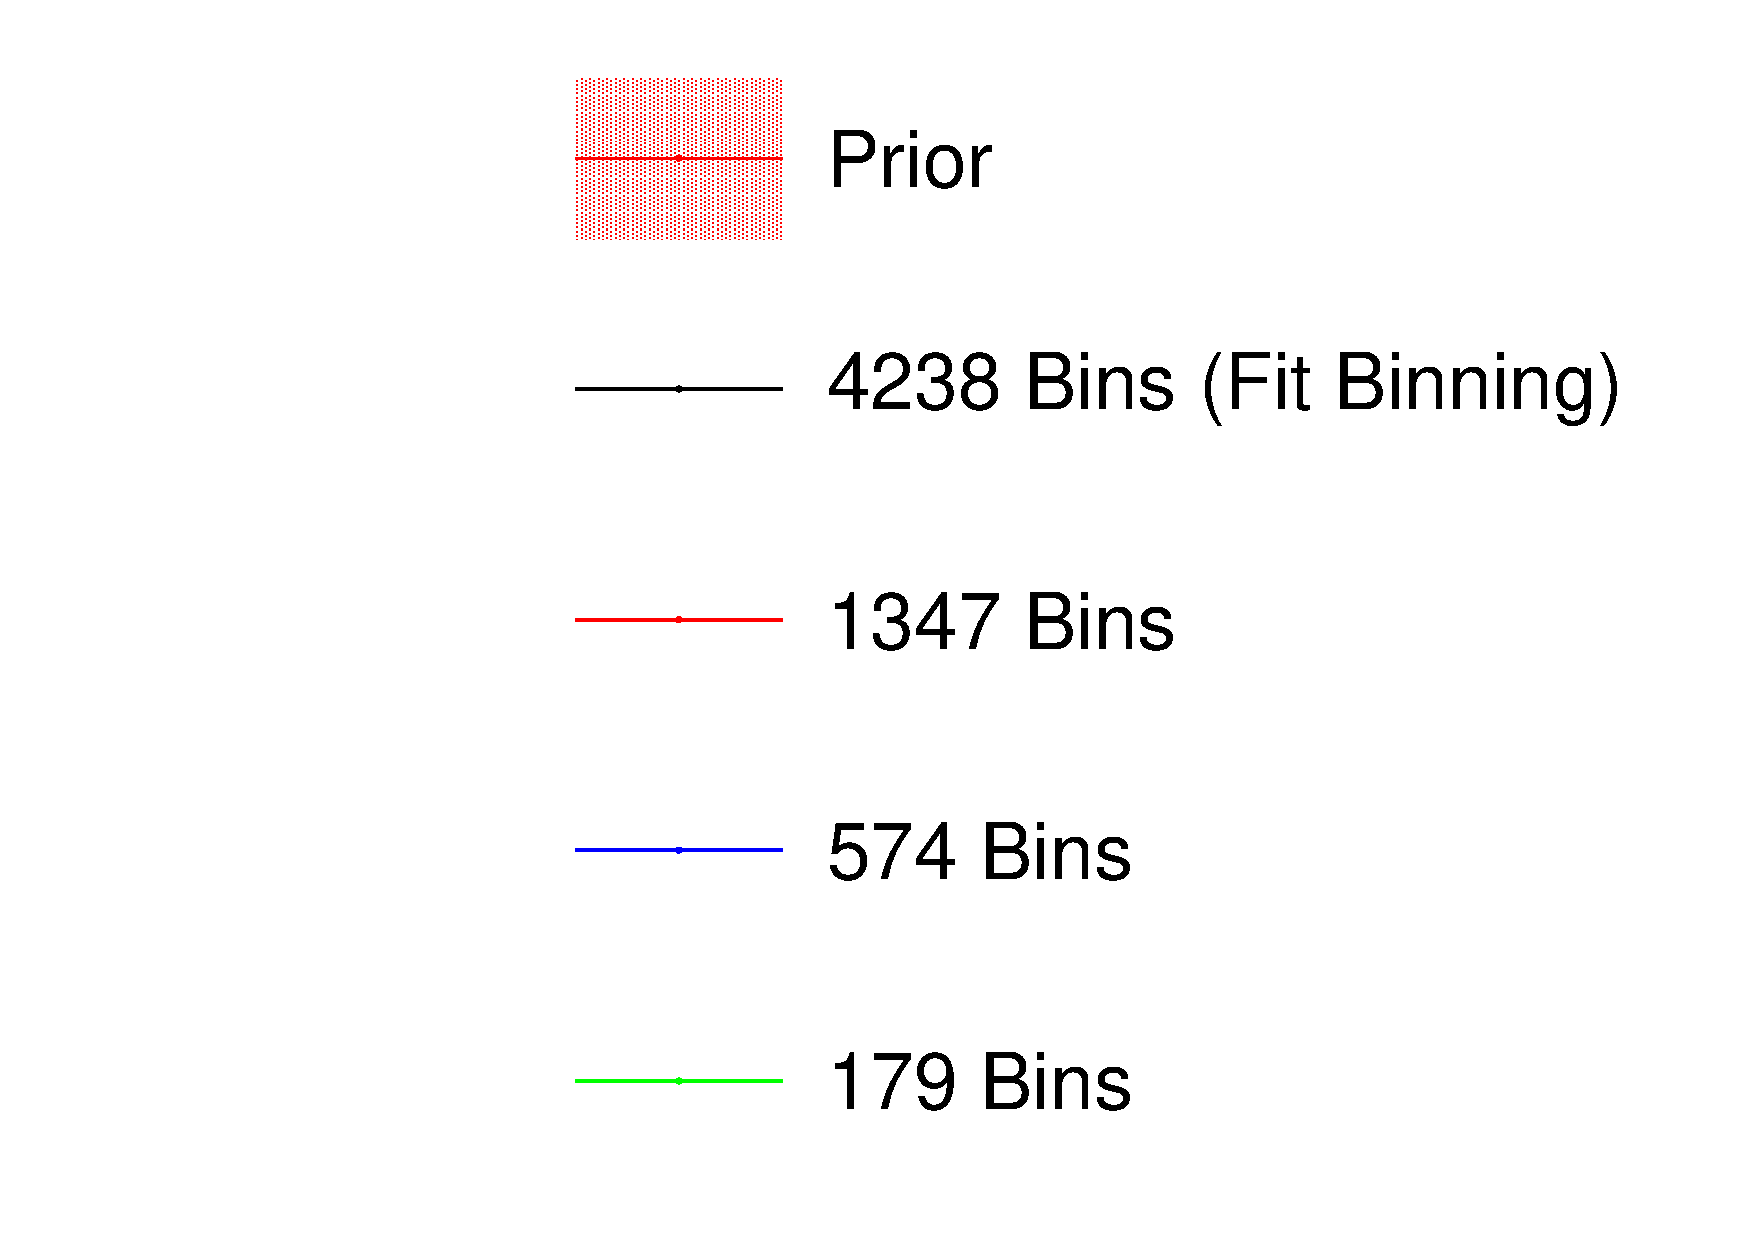
\includegraphics[width=0.8\linewidth, trim={5mm  65mm 0mm 0mm}, clip]{figs/detcovbin_leg}
\end{subfigure}
\begin{subfigure}{0.3\textwidth}
  \centering
  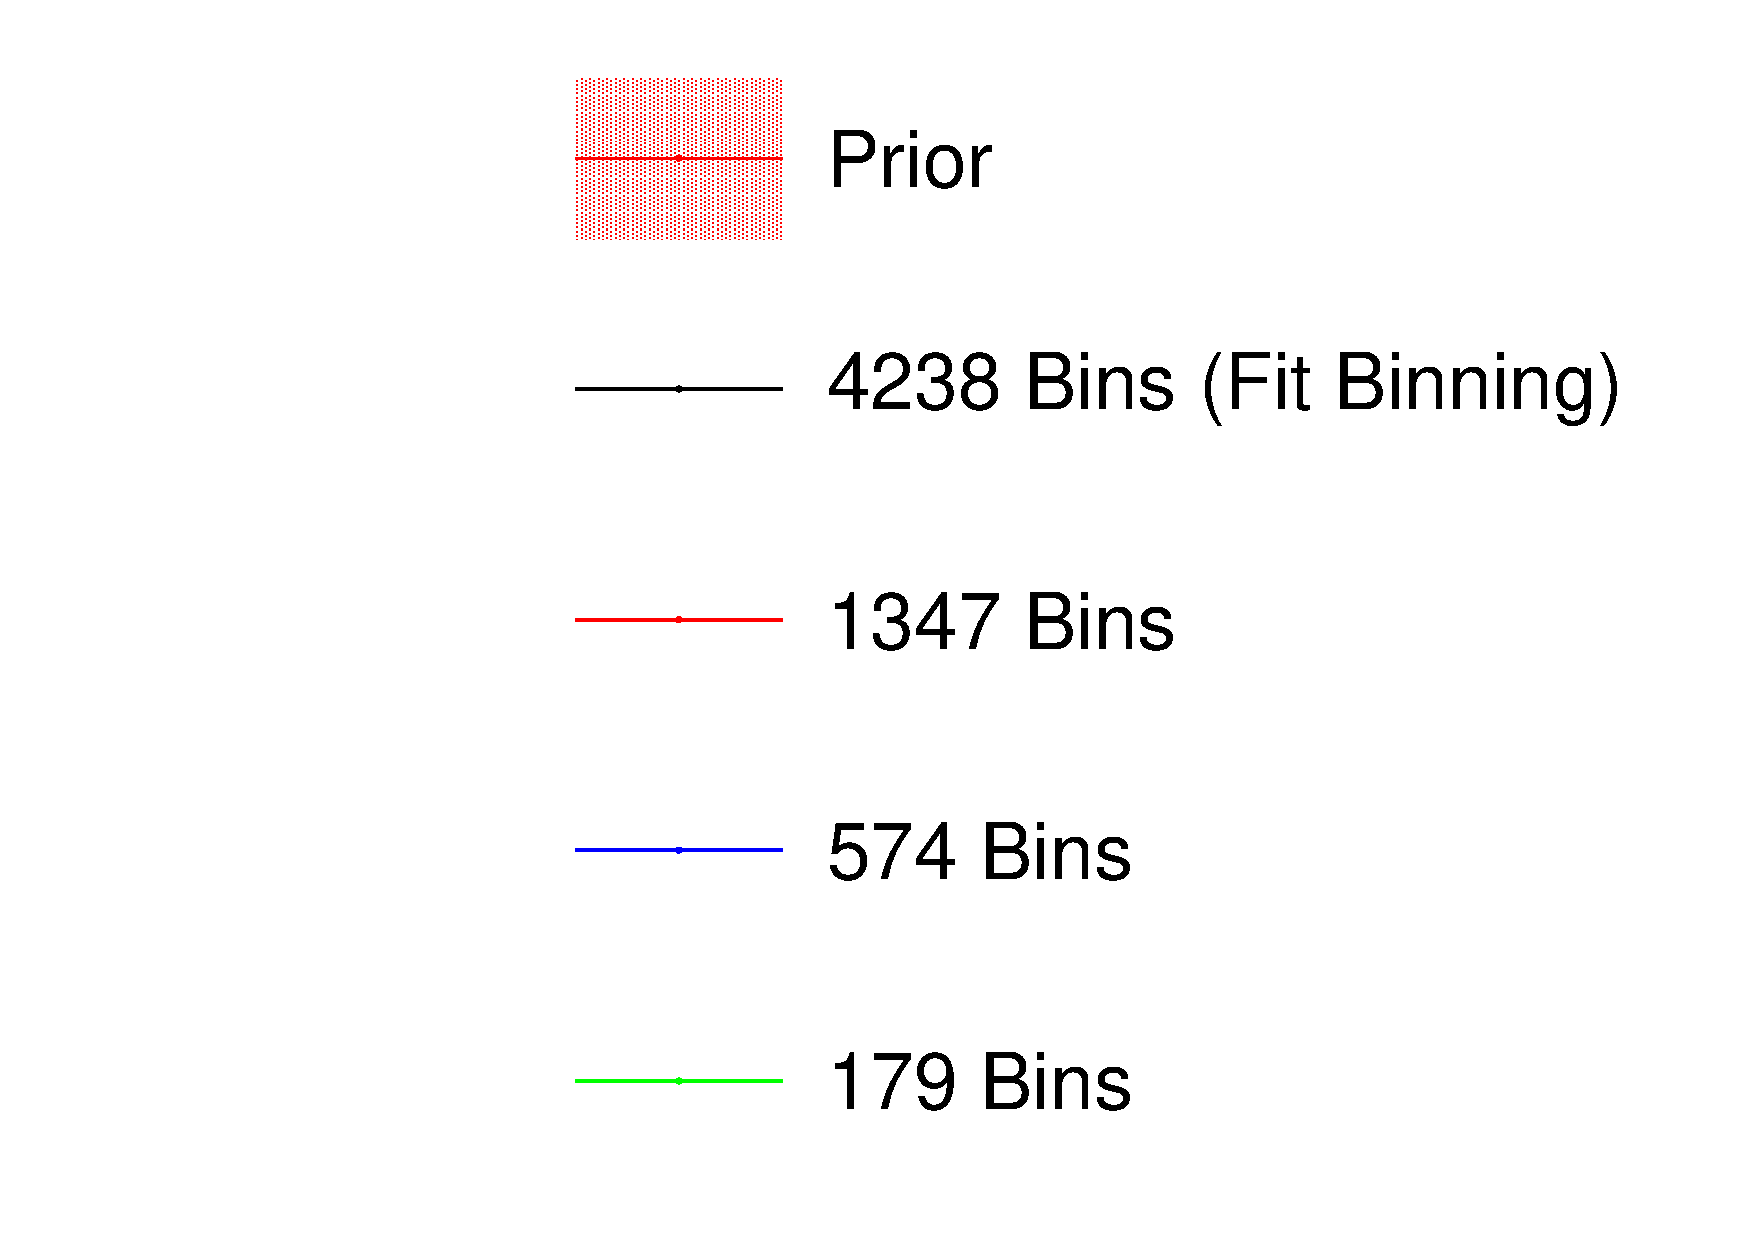
\includegraphics[width=0.8\linewidth, trim={5mm  0mm 0mm 105mm}, clip]{figs/detcovbin_leg}
\end{subfigure}
\begin{subfigure}{0.45\textwidth}
  \centering
  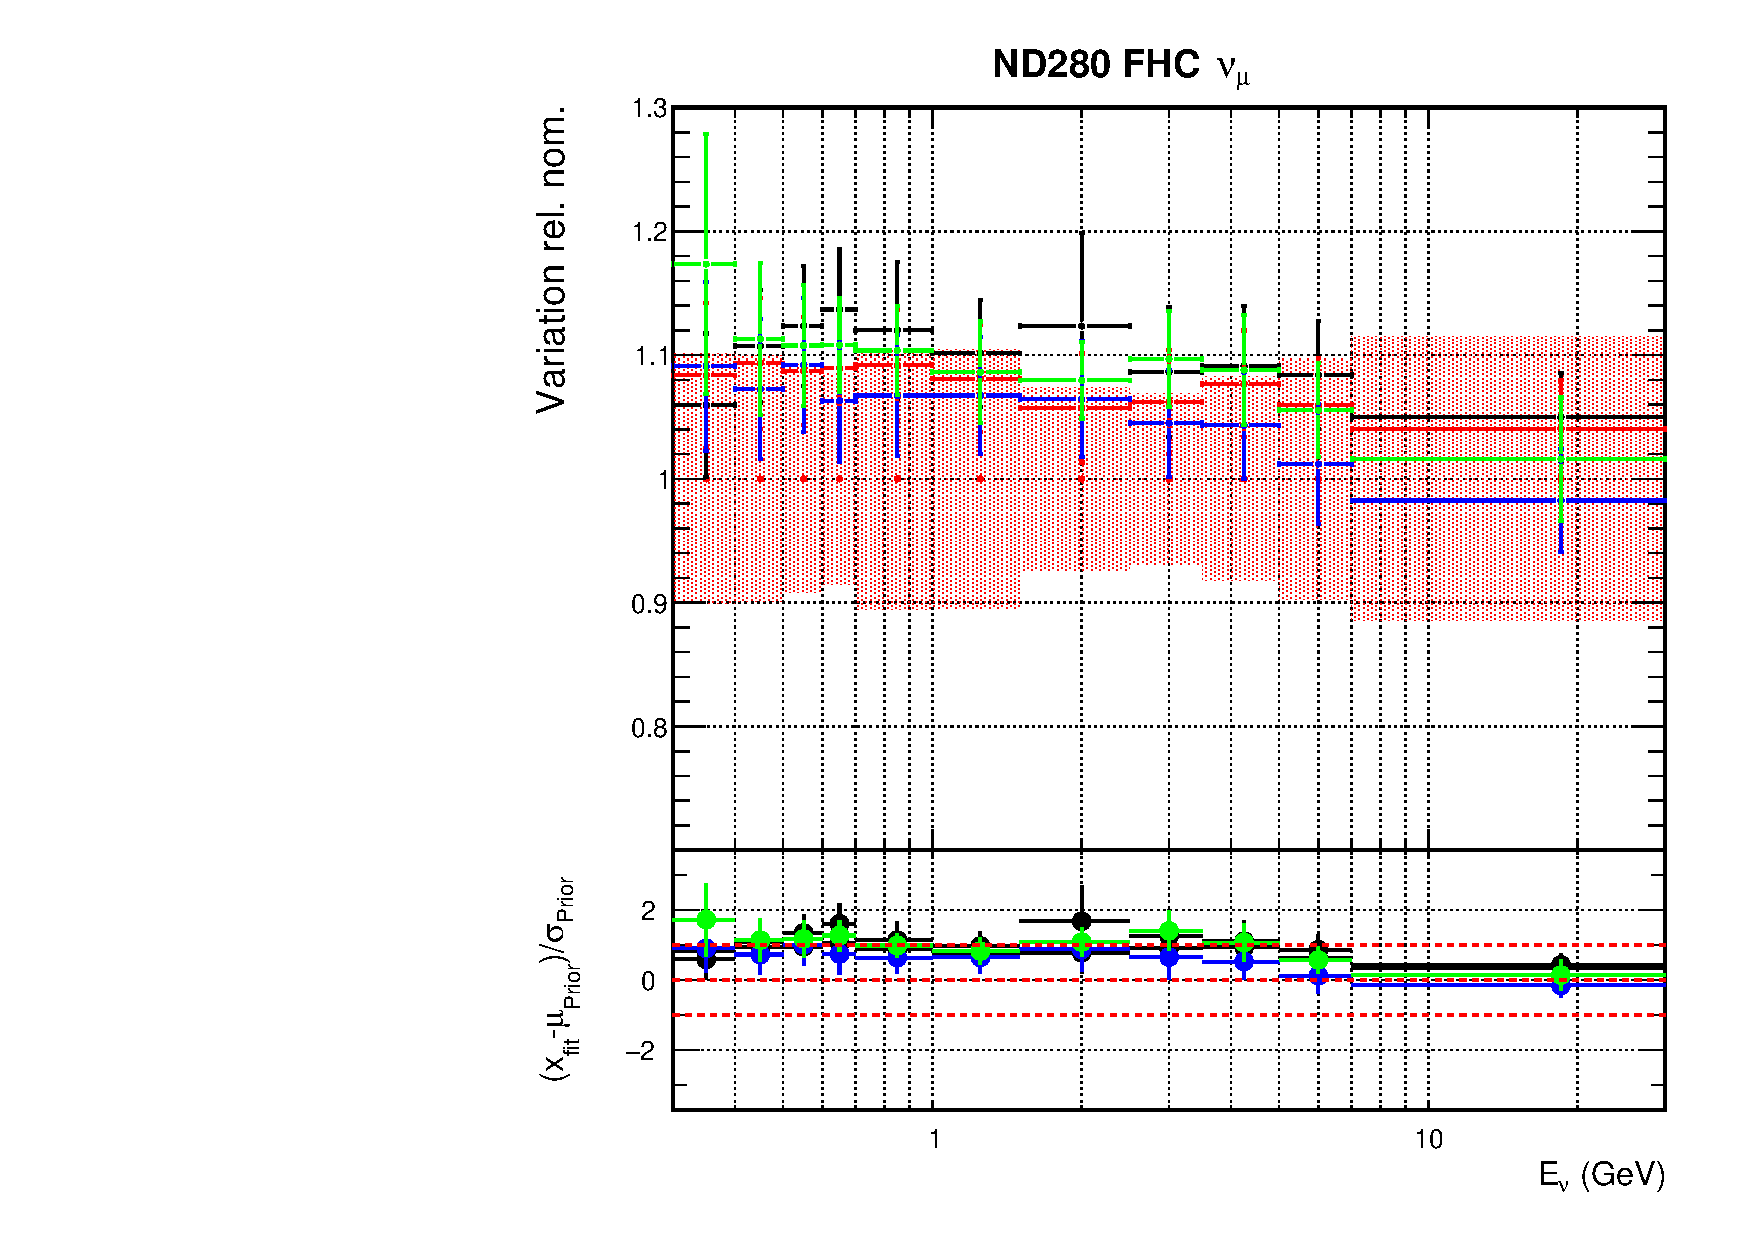
\includegraphics[width=0.75\linewidth]{figs/detcovbinflux_0}
  \caption{ND FHC $\nu_{\mu}$}
\end{subfigure}
\begin{subfigure}{0.45\textwidth}
  \centering
  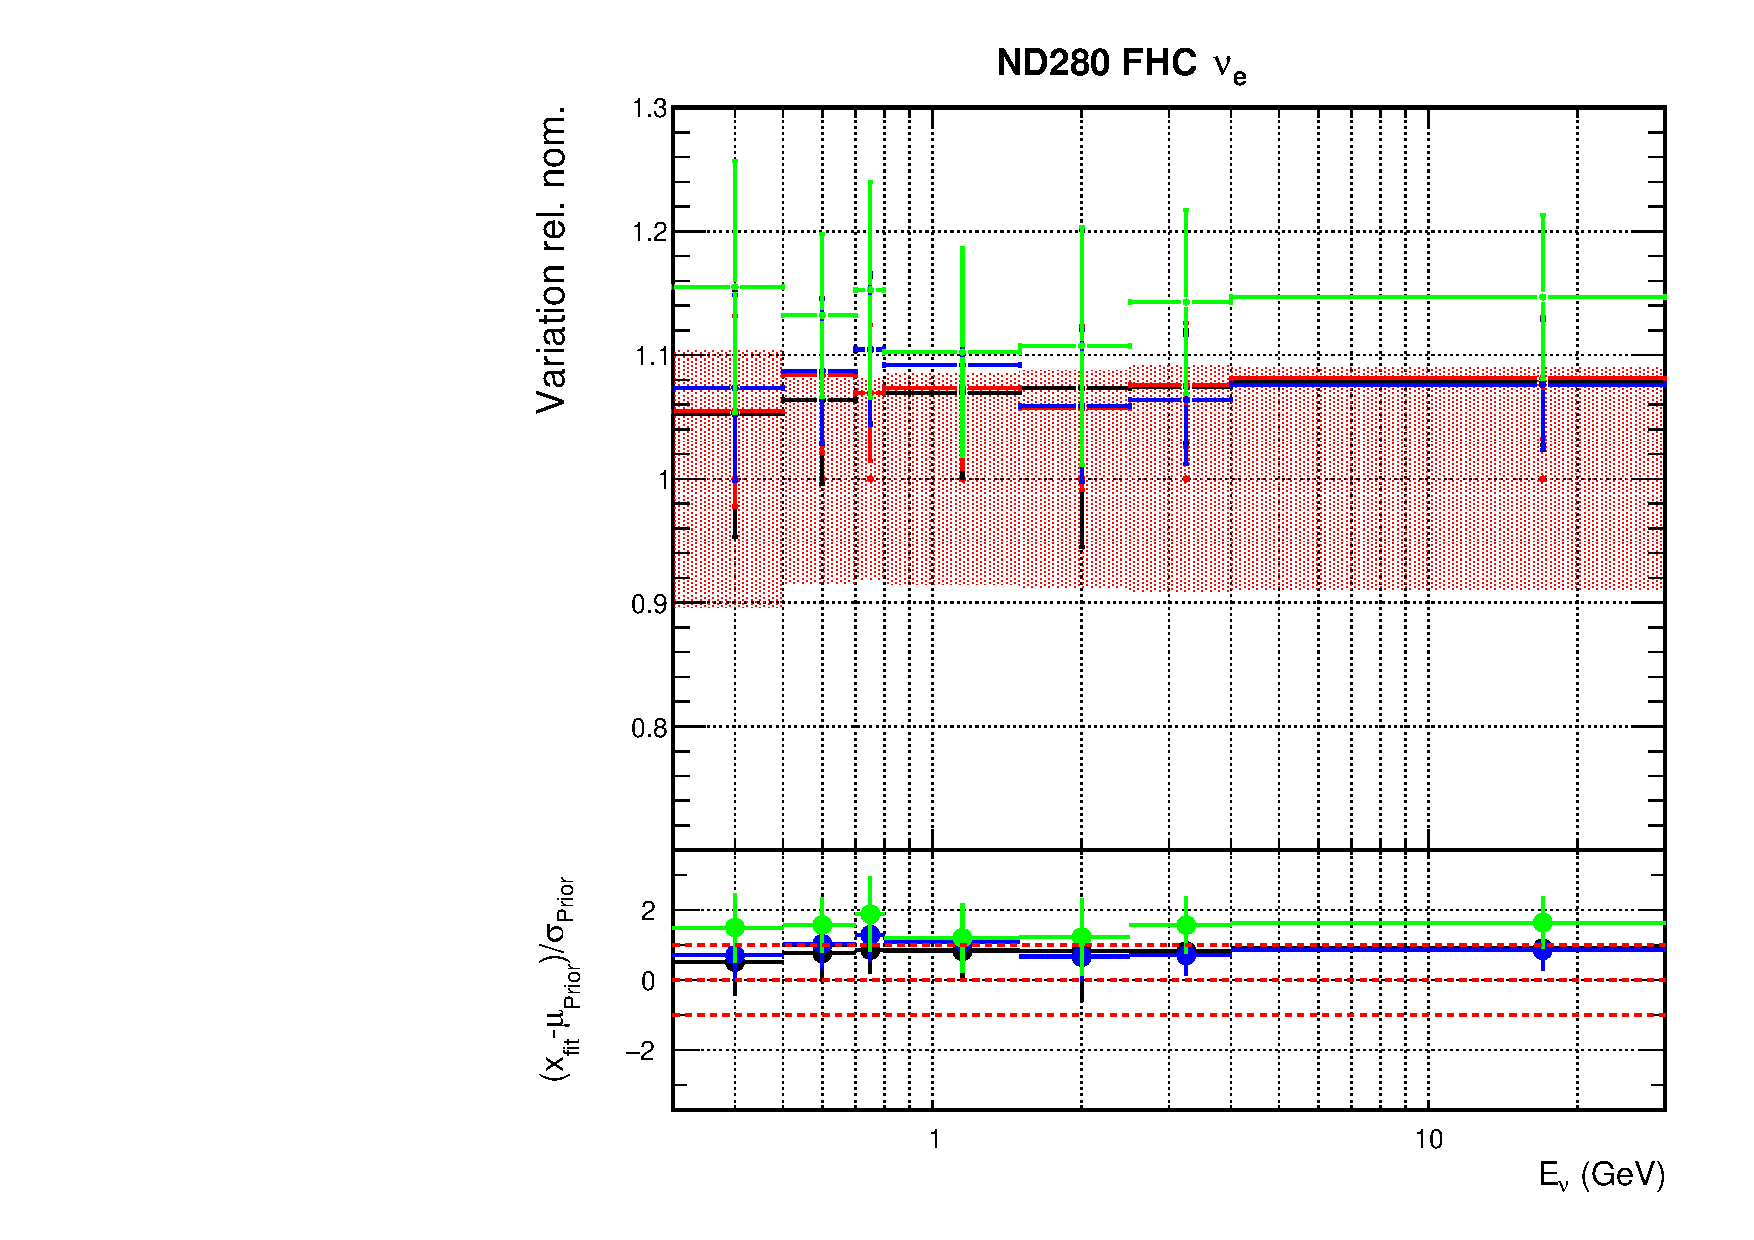
\includegraphics[width=0.75\linewidth]{figs/detcovbinflux_1}
  \caption{ND FHC $\bar{\nu_{\mu}}$}
\end{subfigure}
\begin{subfigure}{0.45\textwidth}
  \centering
  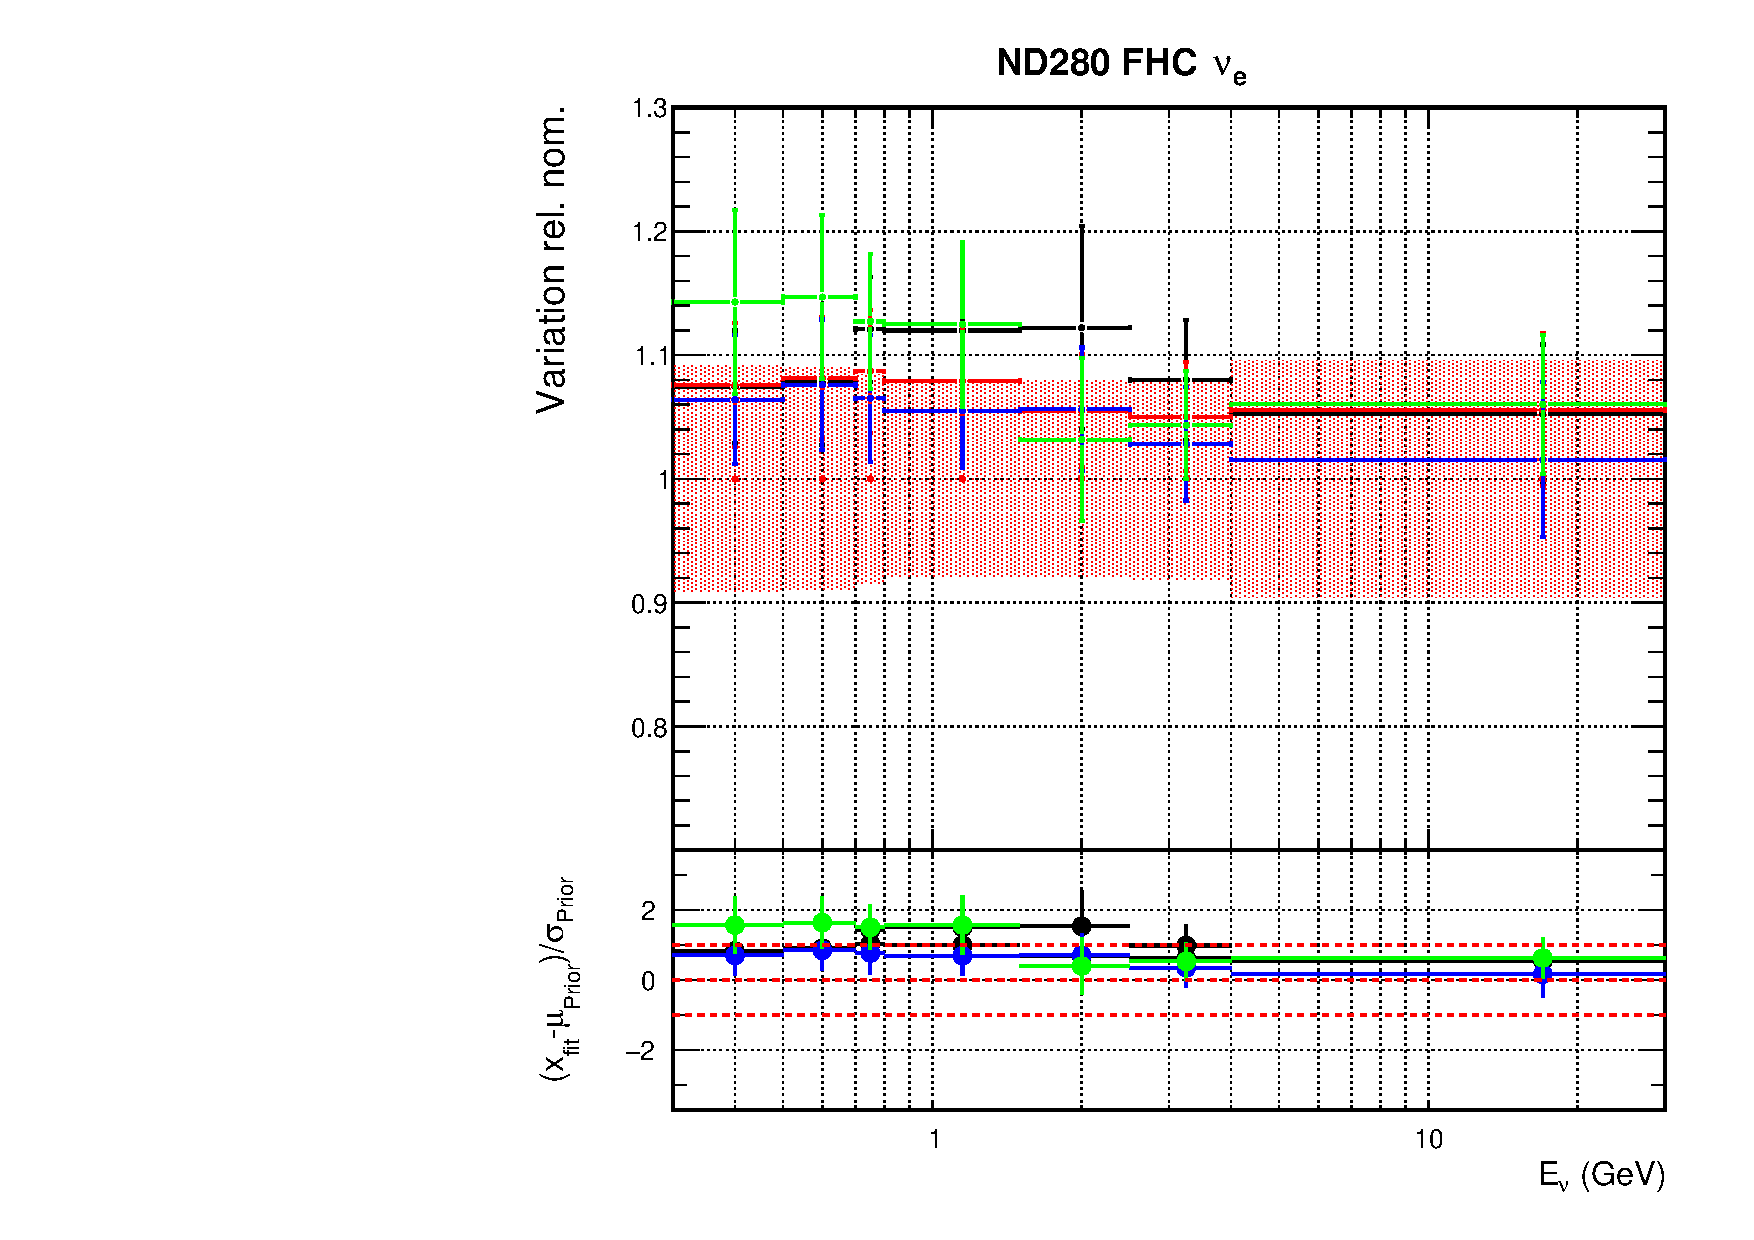
\includegraphics[width=0.75\linewidth]{figs/detcovbinflux_2}
  \caption{ND FHC $\nu_e$}
\end{subfigure}
\begin{subfigure}{0.45\textwidth}
  \centering
  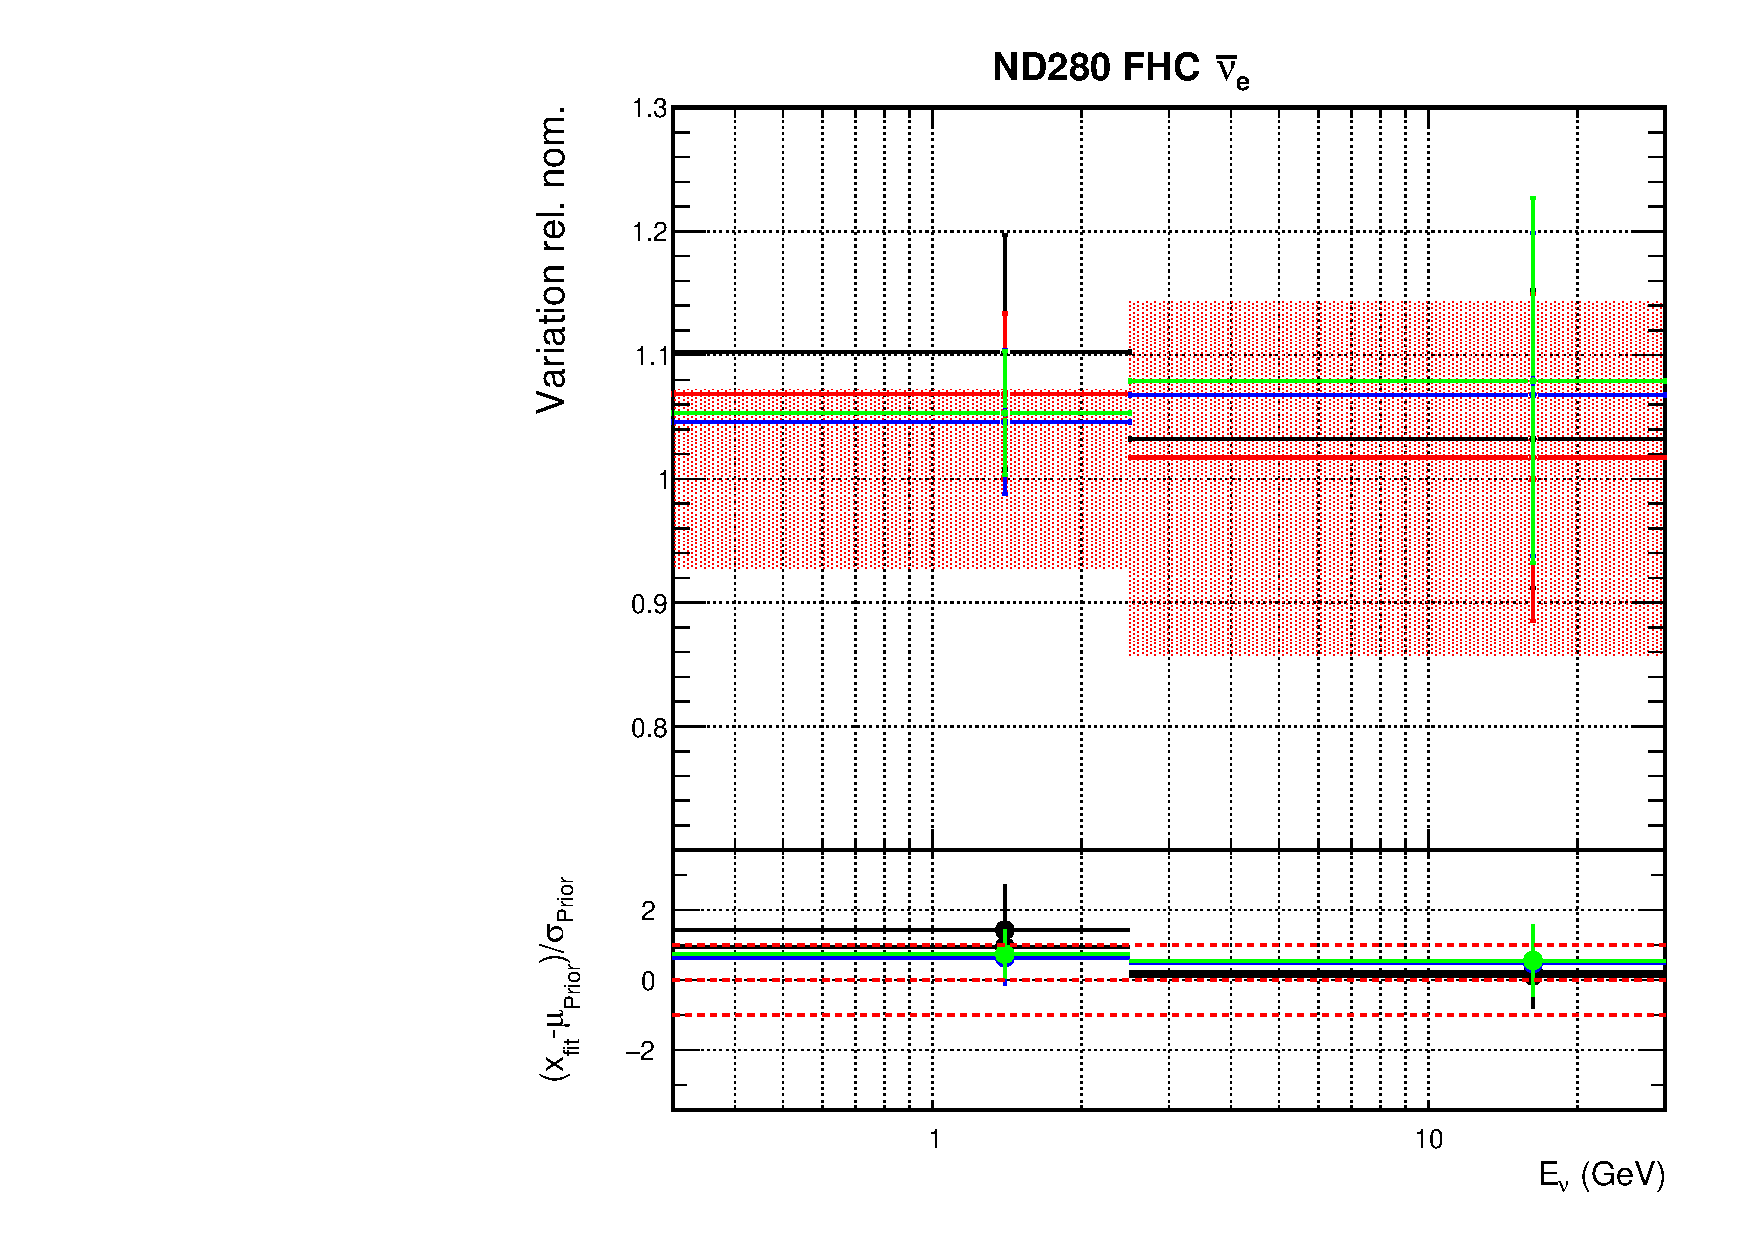
\includegraphics[width=0.75\linewidth]{figs/detcovbinflux_3}
  \caption{ND FHC $\bar{\nu_{e}}$}
\end{subfigure}
\begin{subfigure}{0.45\textwidth}
  \centering
  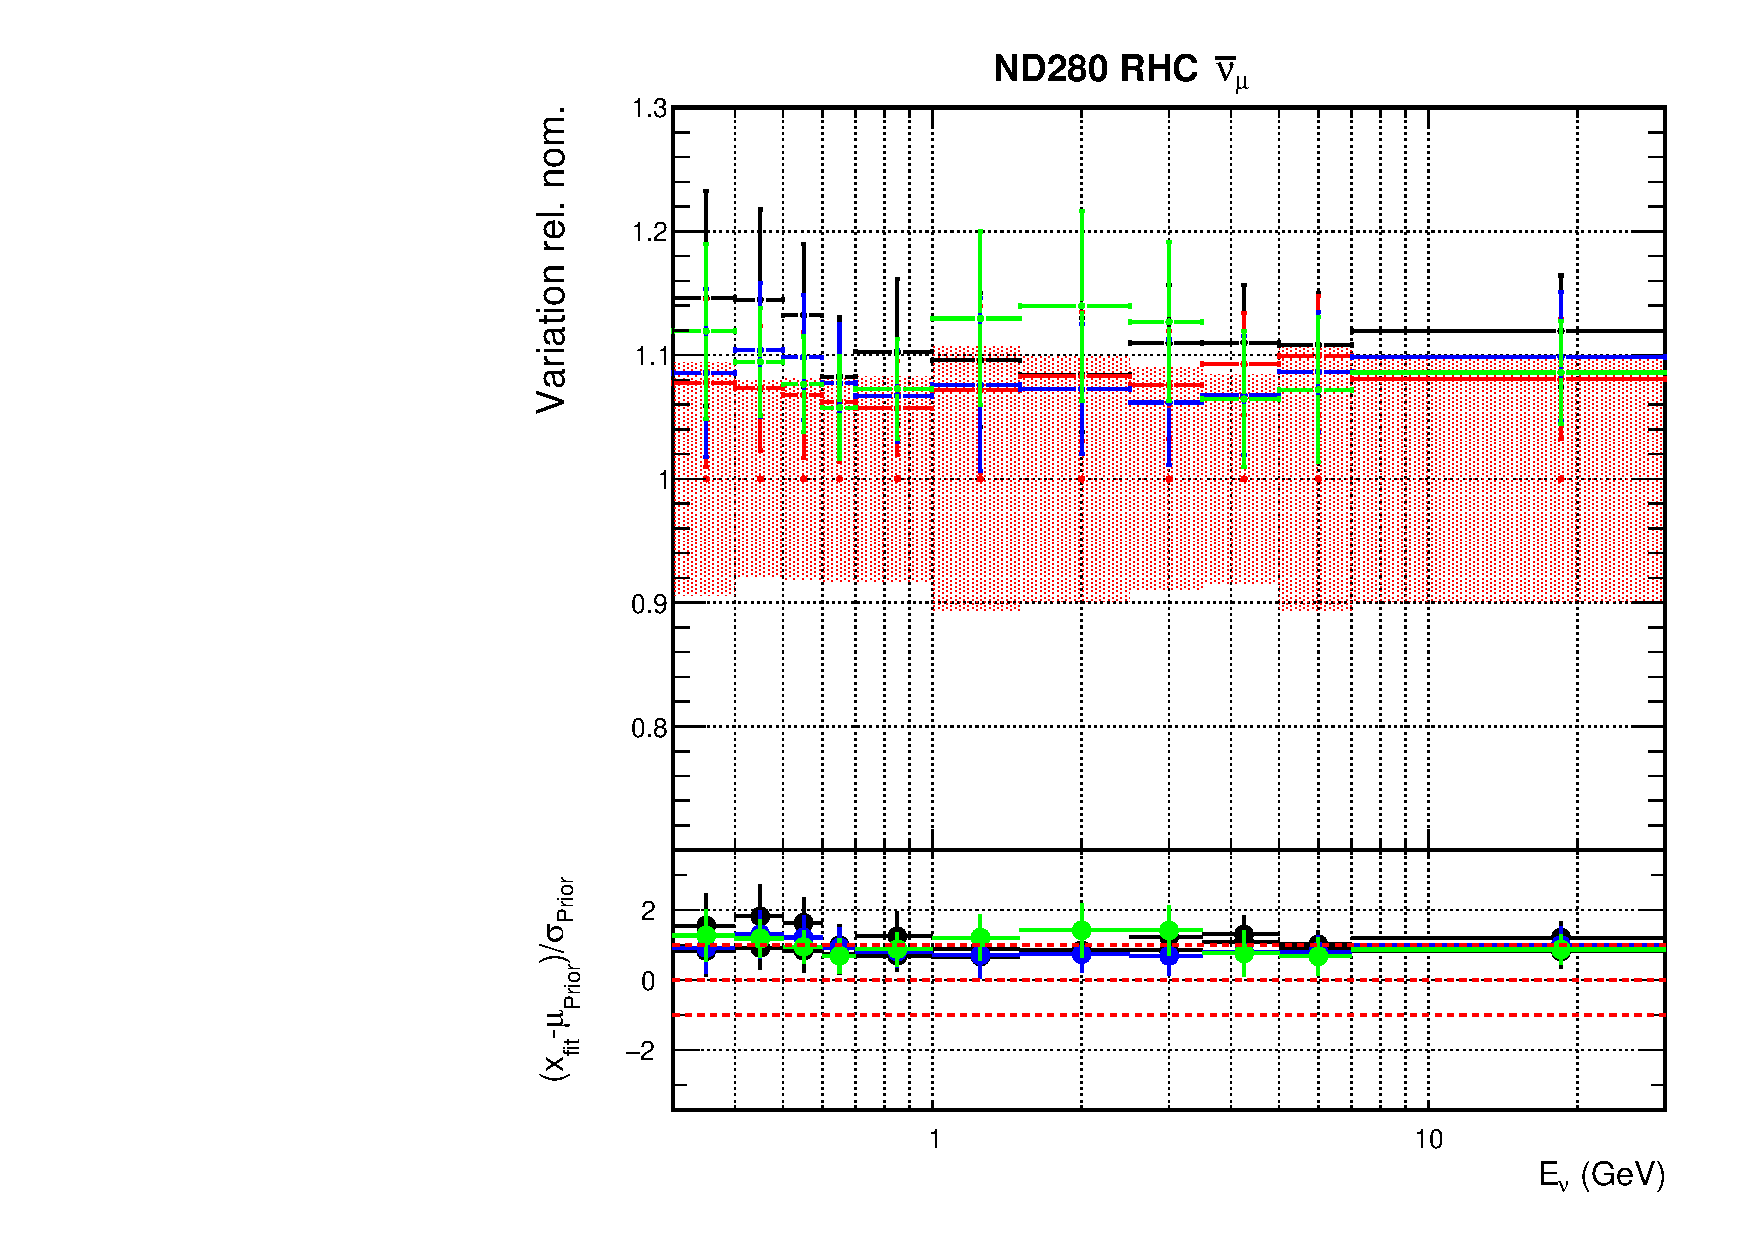
\includegraphics[width=0.75\linewidth]{figs/detcovbinflux_4}
  \caption{ND RHC $\nu_{\mu}$}
\end{subfigure}
\begin{subfigure}{0.45\textwidth}
  \centering
  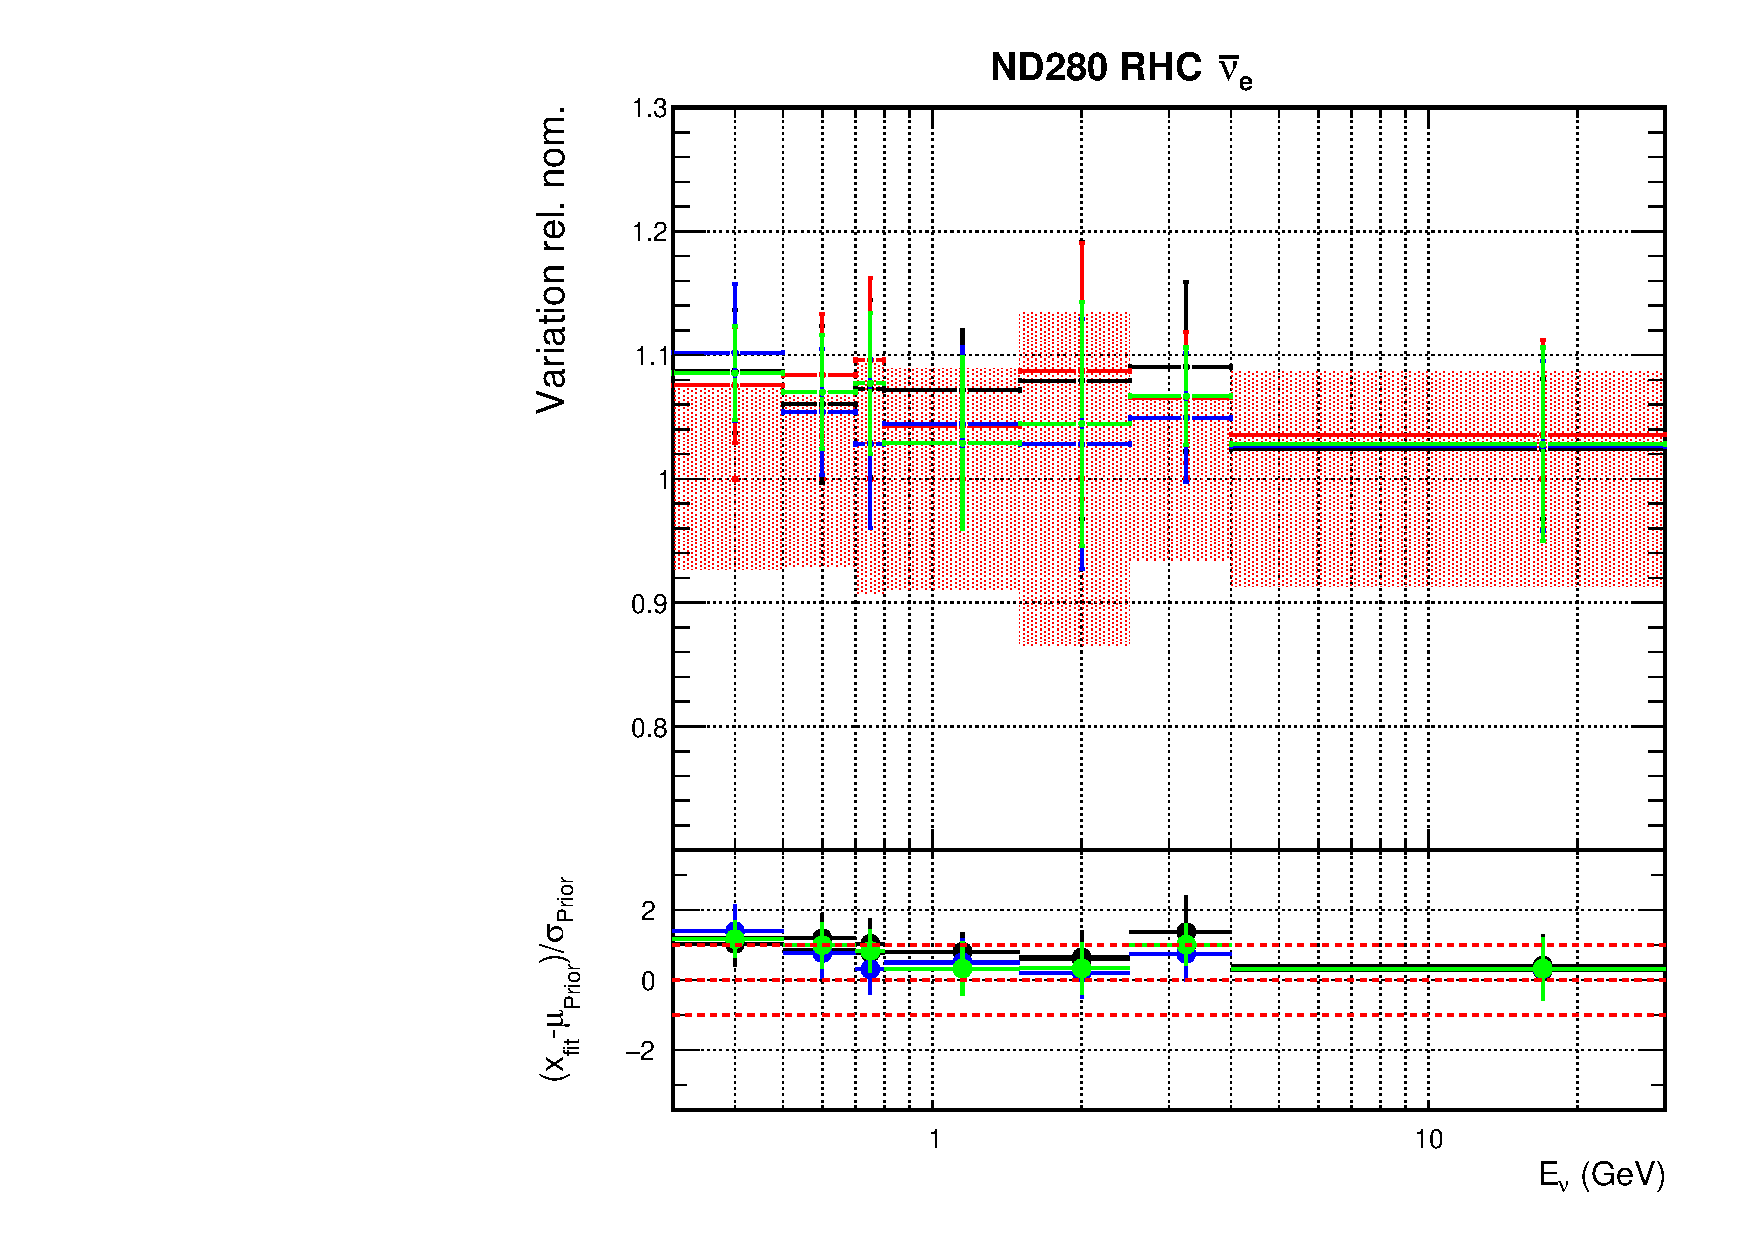
\includegraphics[width=0.75\linewidth]{figs/detcovbinflux_5}
  \caption{ND RHC $\bar{\nu_{\mu}}$}
\end{subfigure}
\begin{subfigure}{0.45\textwidth}
  \centering
  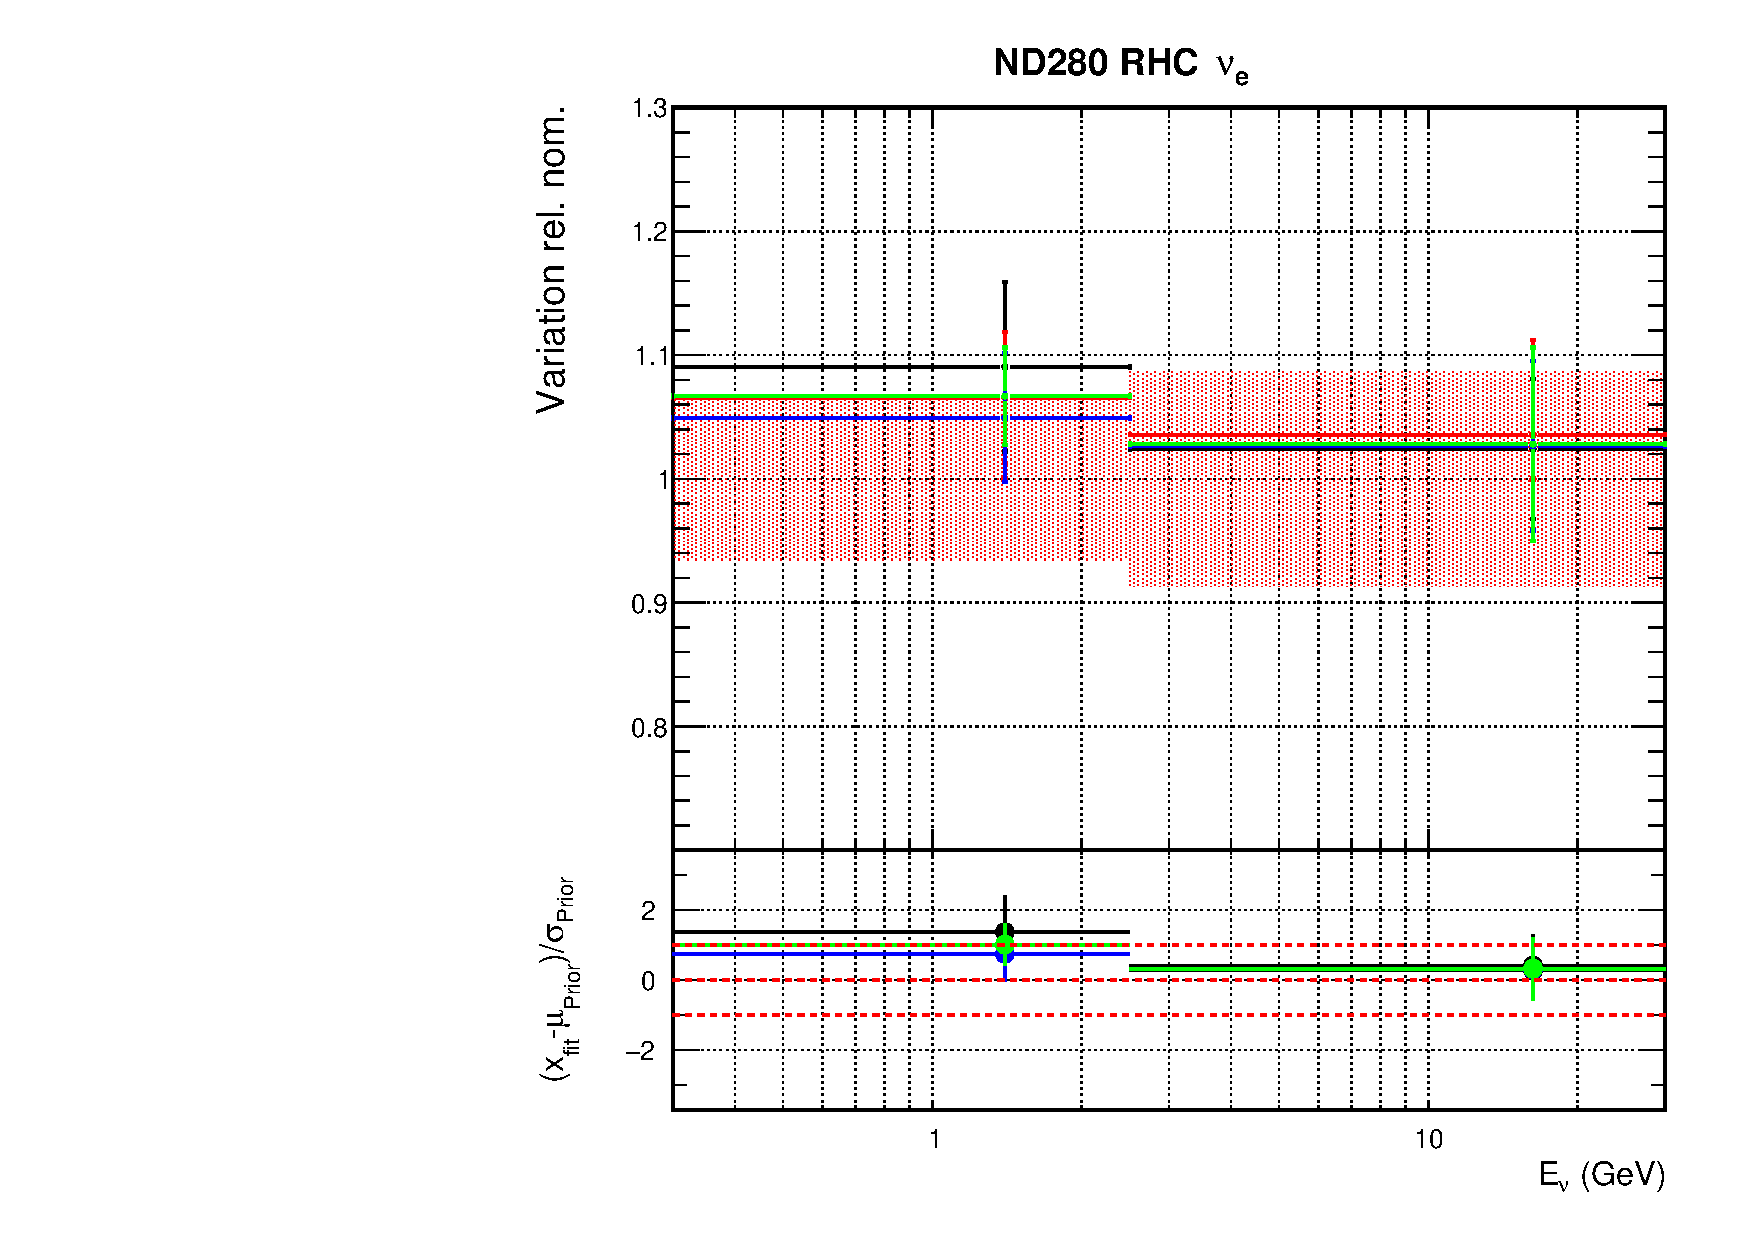
\includegraphics[width=0.75\linewidth]{figs/detcovbinflux_6}
  \caption{ND RHC $\nu_e$}
\end{subfigure}
\begin{subfigure}{0.45\textwidth}
  \centering
  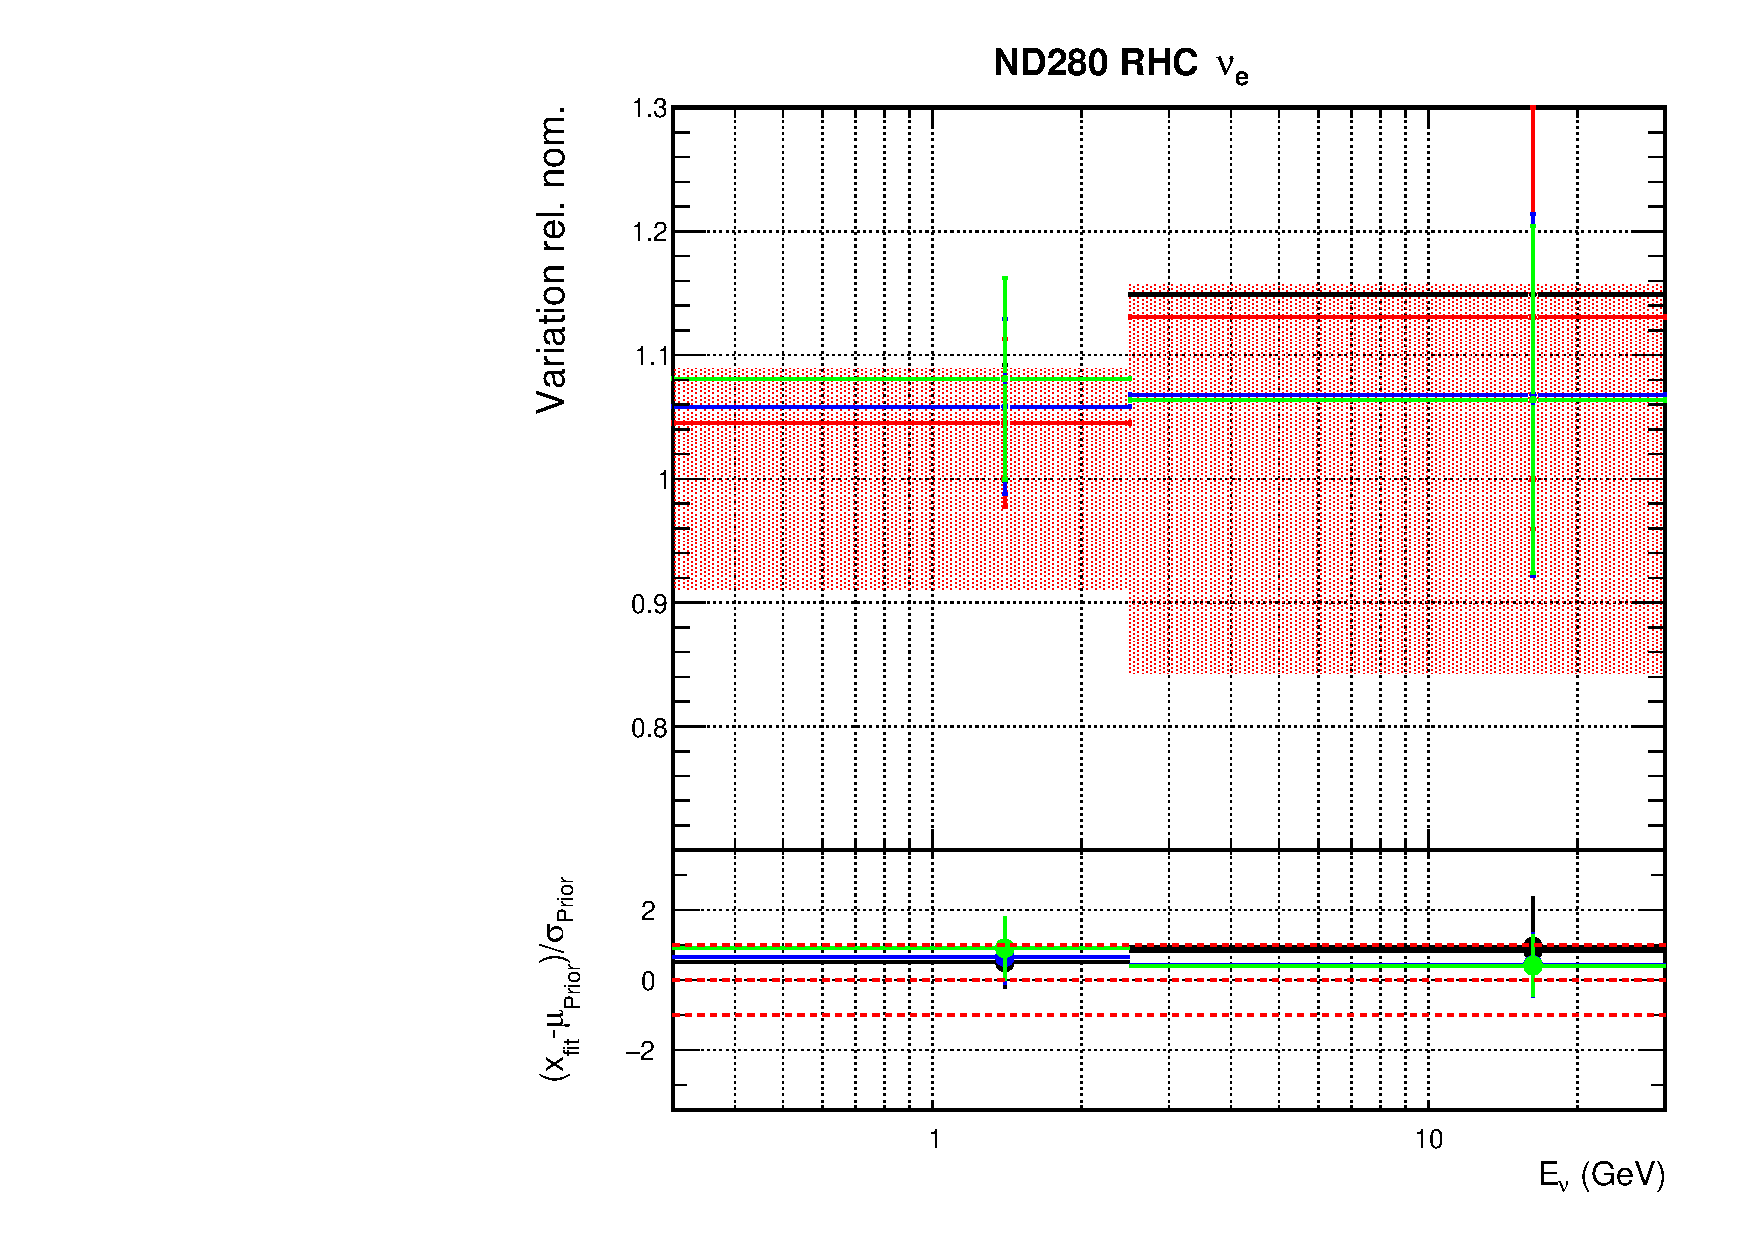
\includegraphics[width=0.75\linewidth]{figs/detcovbinflux_7}
  \caption{ND RHC $\bar{\nu_e}$}
\end{subfigure}
\caption{ND280 flux parameters for fake data fits using different detector binnings.}
\label{fig:detcovbinfluxNDapp}
\end{figure}

\begin{figure}[!htbp]
\centering
\begin{subfigure}{0.3\textwidth}
  \centering
  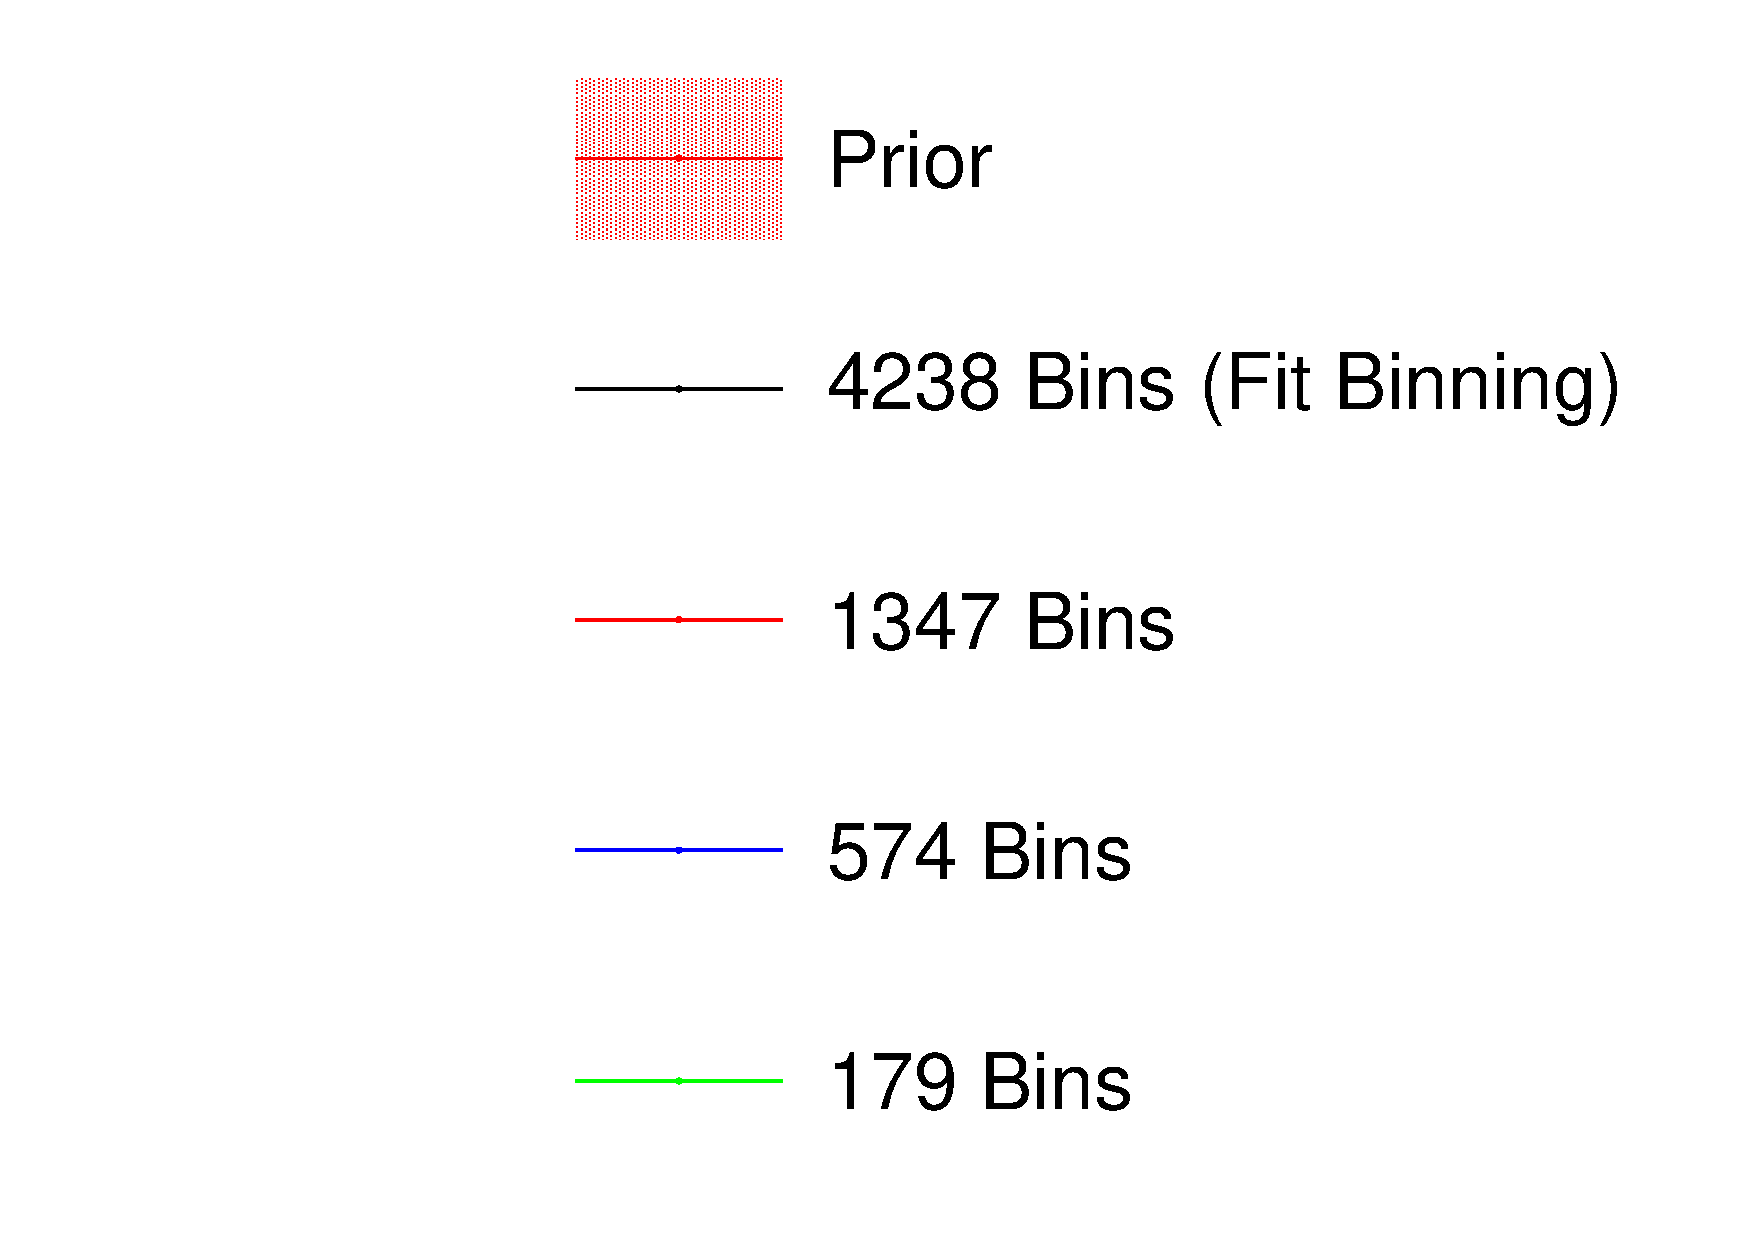
\includegraphics[width=0.8\linewidth, trim={5mm  65mm 0mm 0mm}, clip]{figs/detcovbin_leg}
\end{subfigure}
\begin{subfigure}{0.3\textwidth}
  \centering
  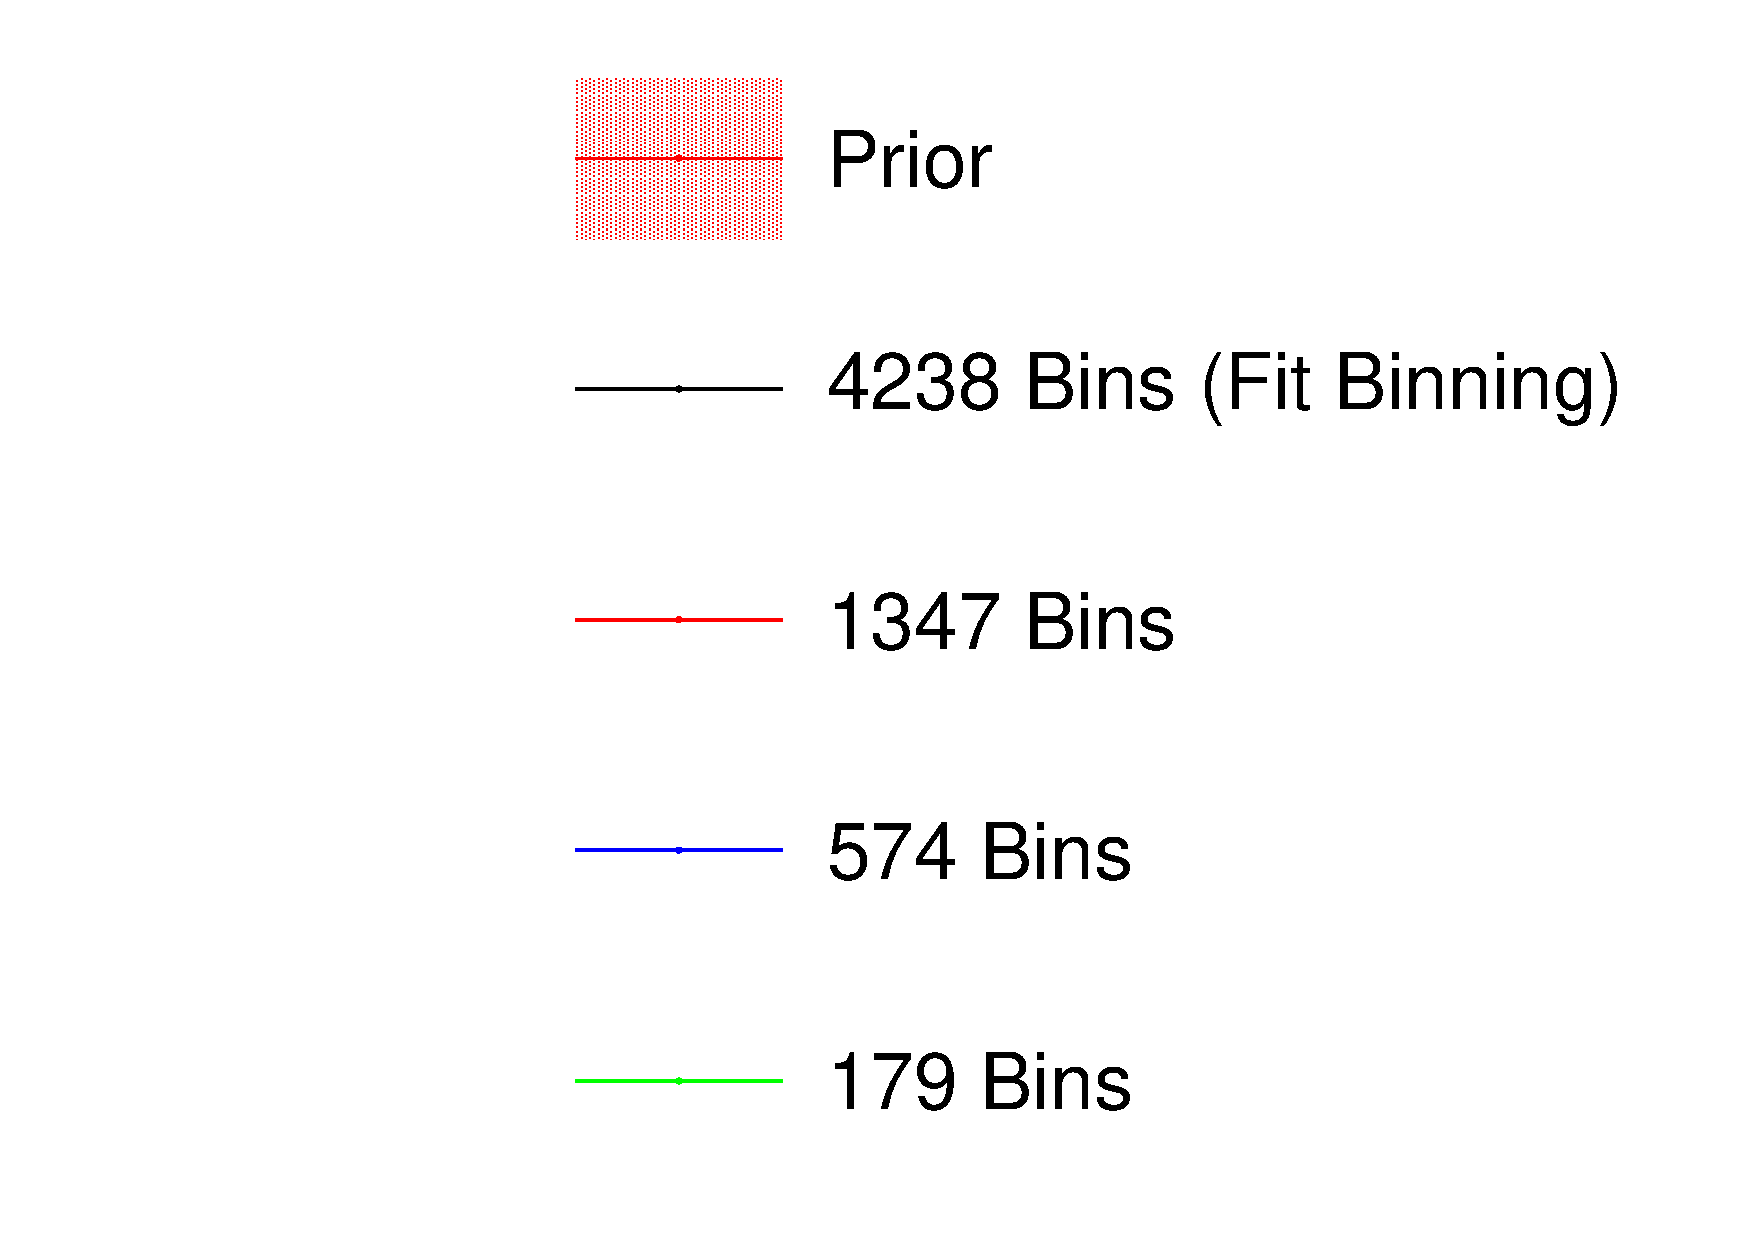
\includegraphics[width=0.8\linewidth, trim={5mm  0mm 0mm 105mm}, clip]{figs/detcovbin_leg}
\end{subfigure}
\begin{subfigure}{0.45\textwidth}
  \centering
  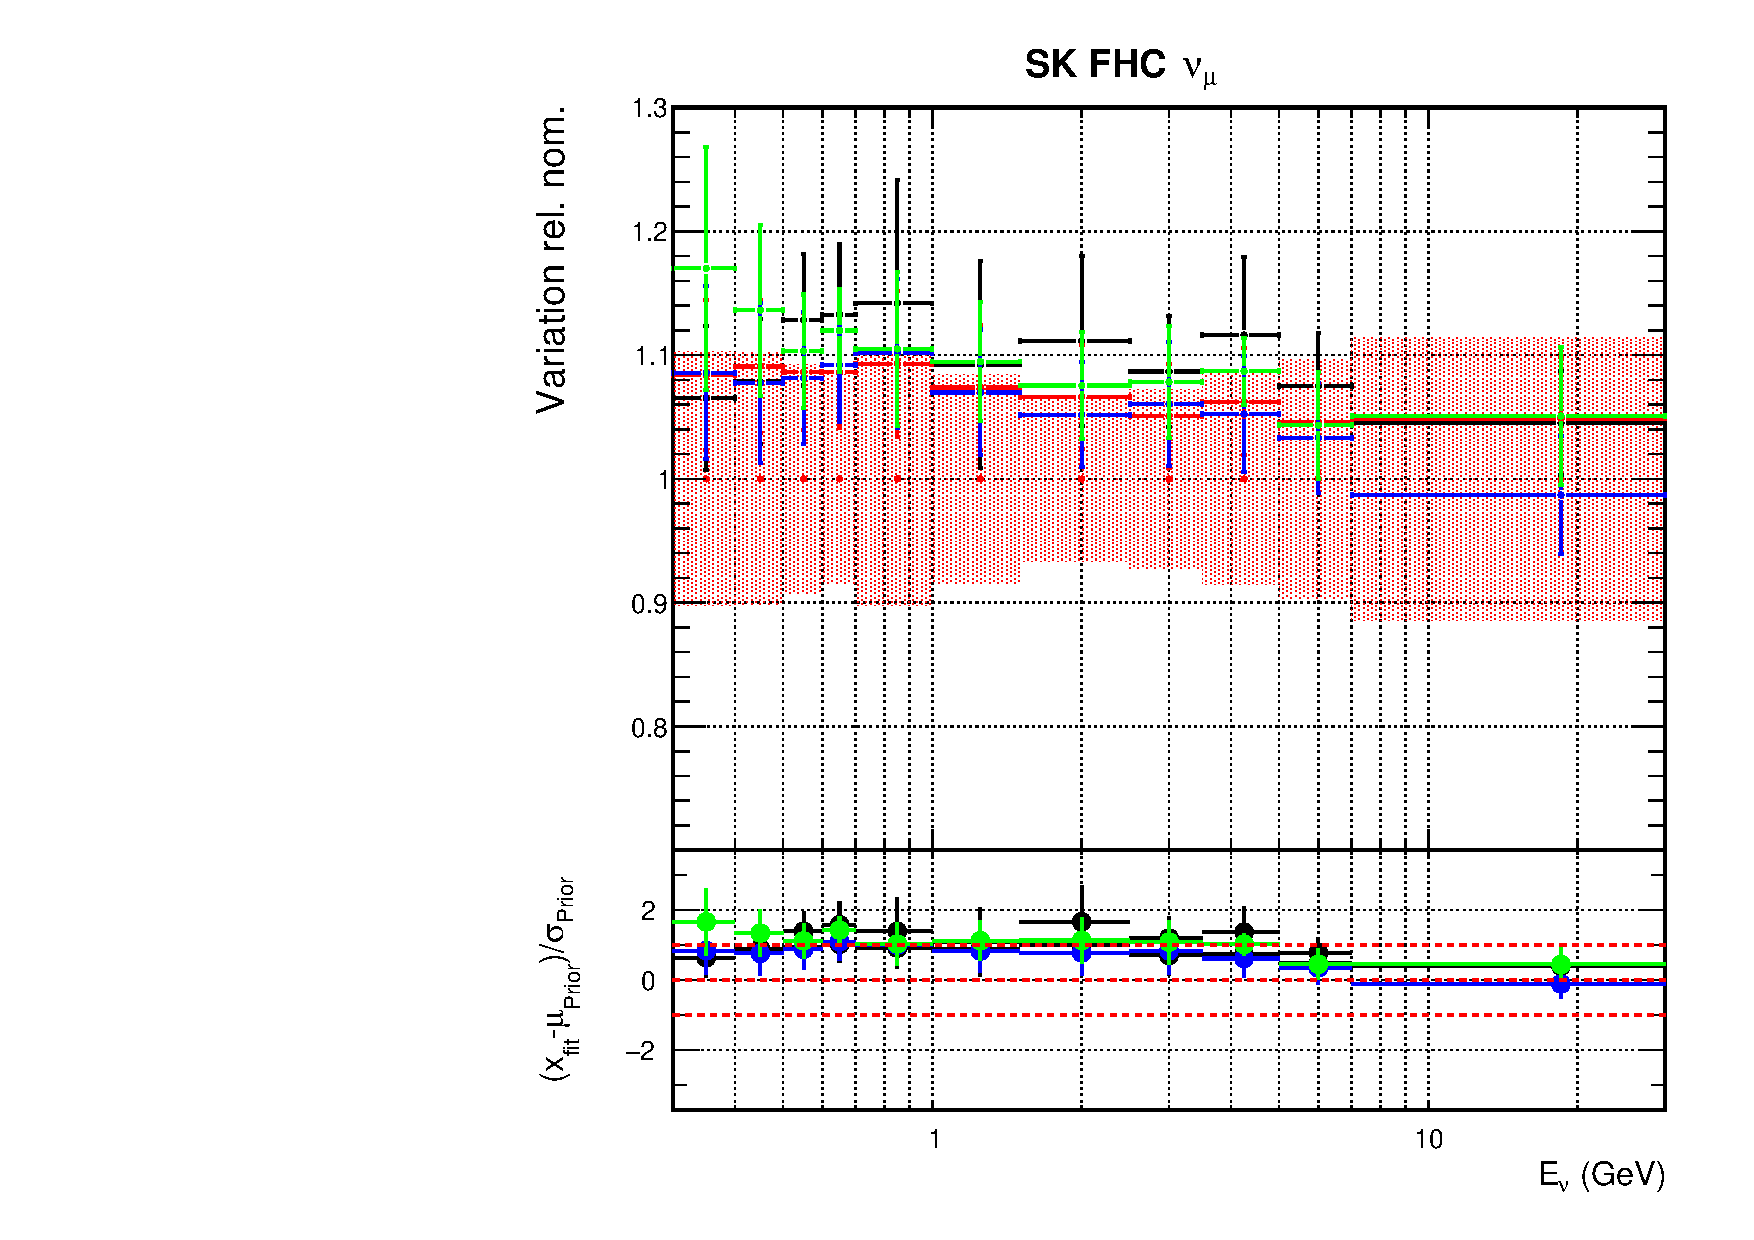
\includegraphics[width=0.75\linewidth]{figs/detcovbinflux_8}
  \caption{SK FHC $\nu_{\mu}$}
\end{subfigure}
\begin{subfigure}{0.45\textwidth}
  \centering
  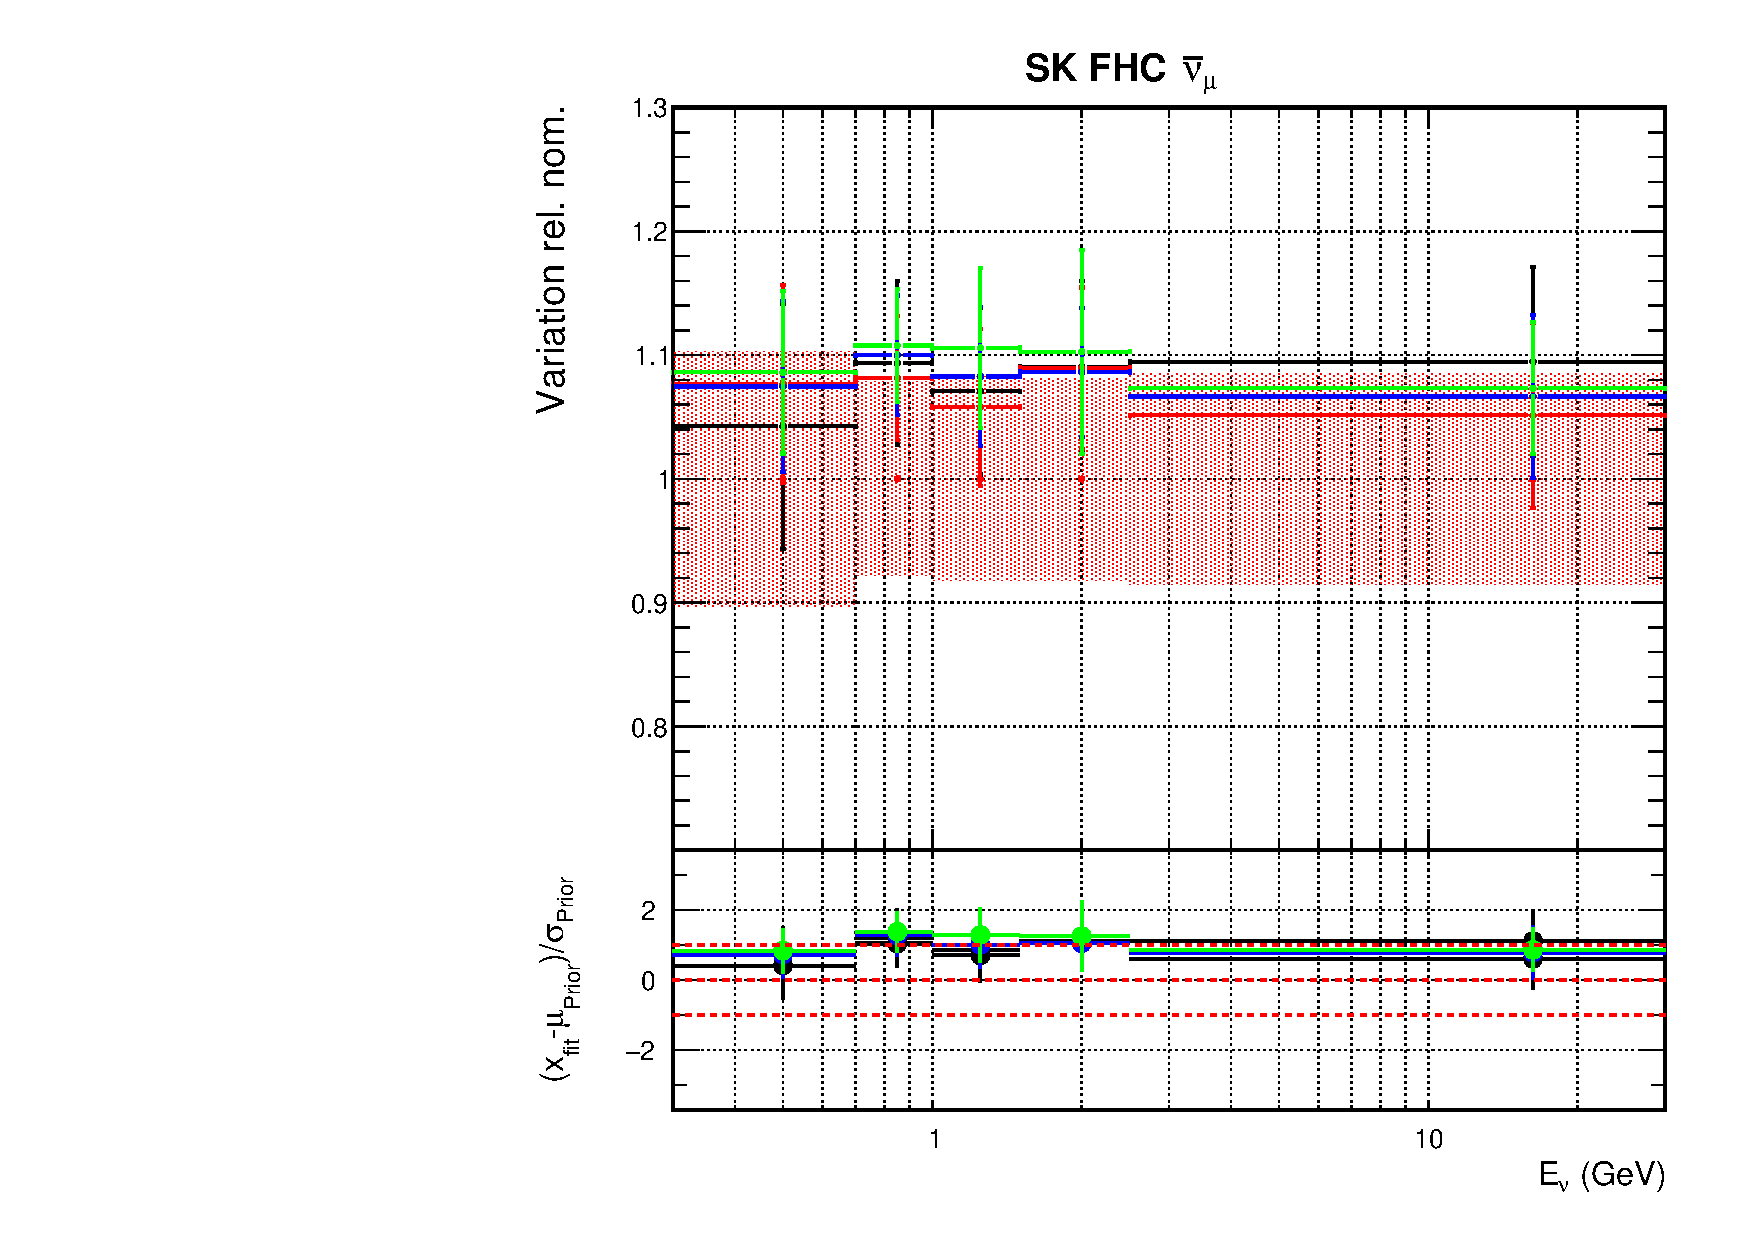
\includegraphics[width=0.75\linewidth]{figs/detcovbinflux_9}
  \caption{SK FHC $\bar{\nu_{\mu}}$}
\end{subfigure}
\begin{subfigure}{0.45\textwidth}
  \centering
  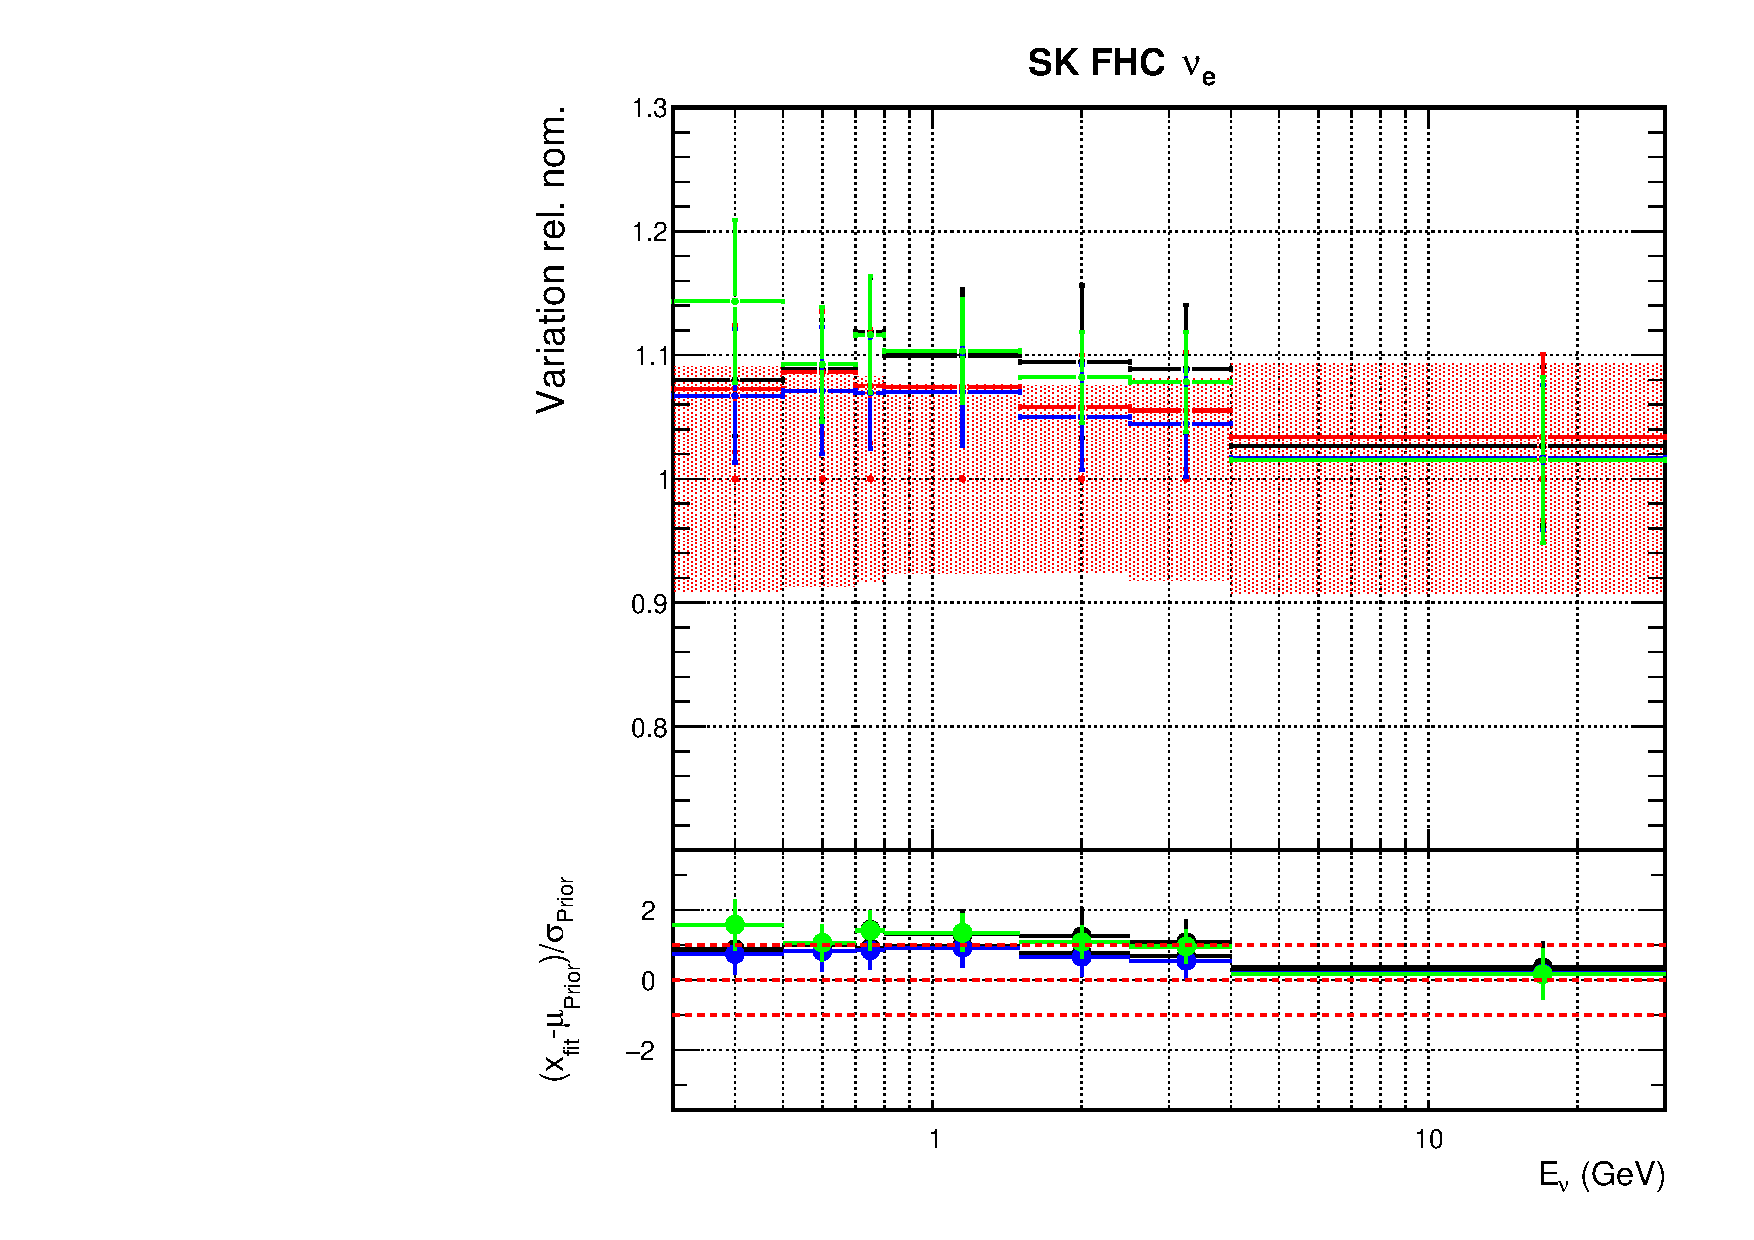
\includegraphics[width=0.75\linewidth]{figs/detcovbinflux_10}
  \caption{SK FHC $\nu_e$}
\end{subfigure}
\begin{subfigure}{0.45\textwidth}
  \centering
  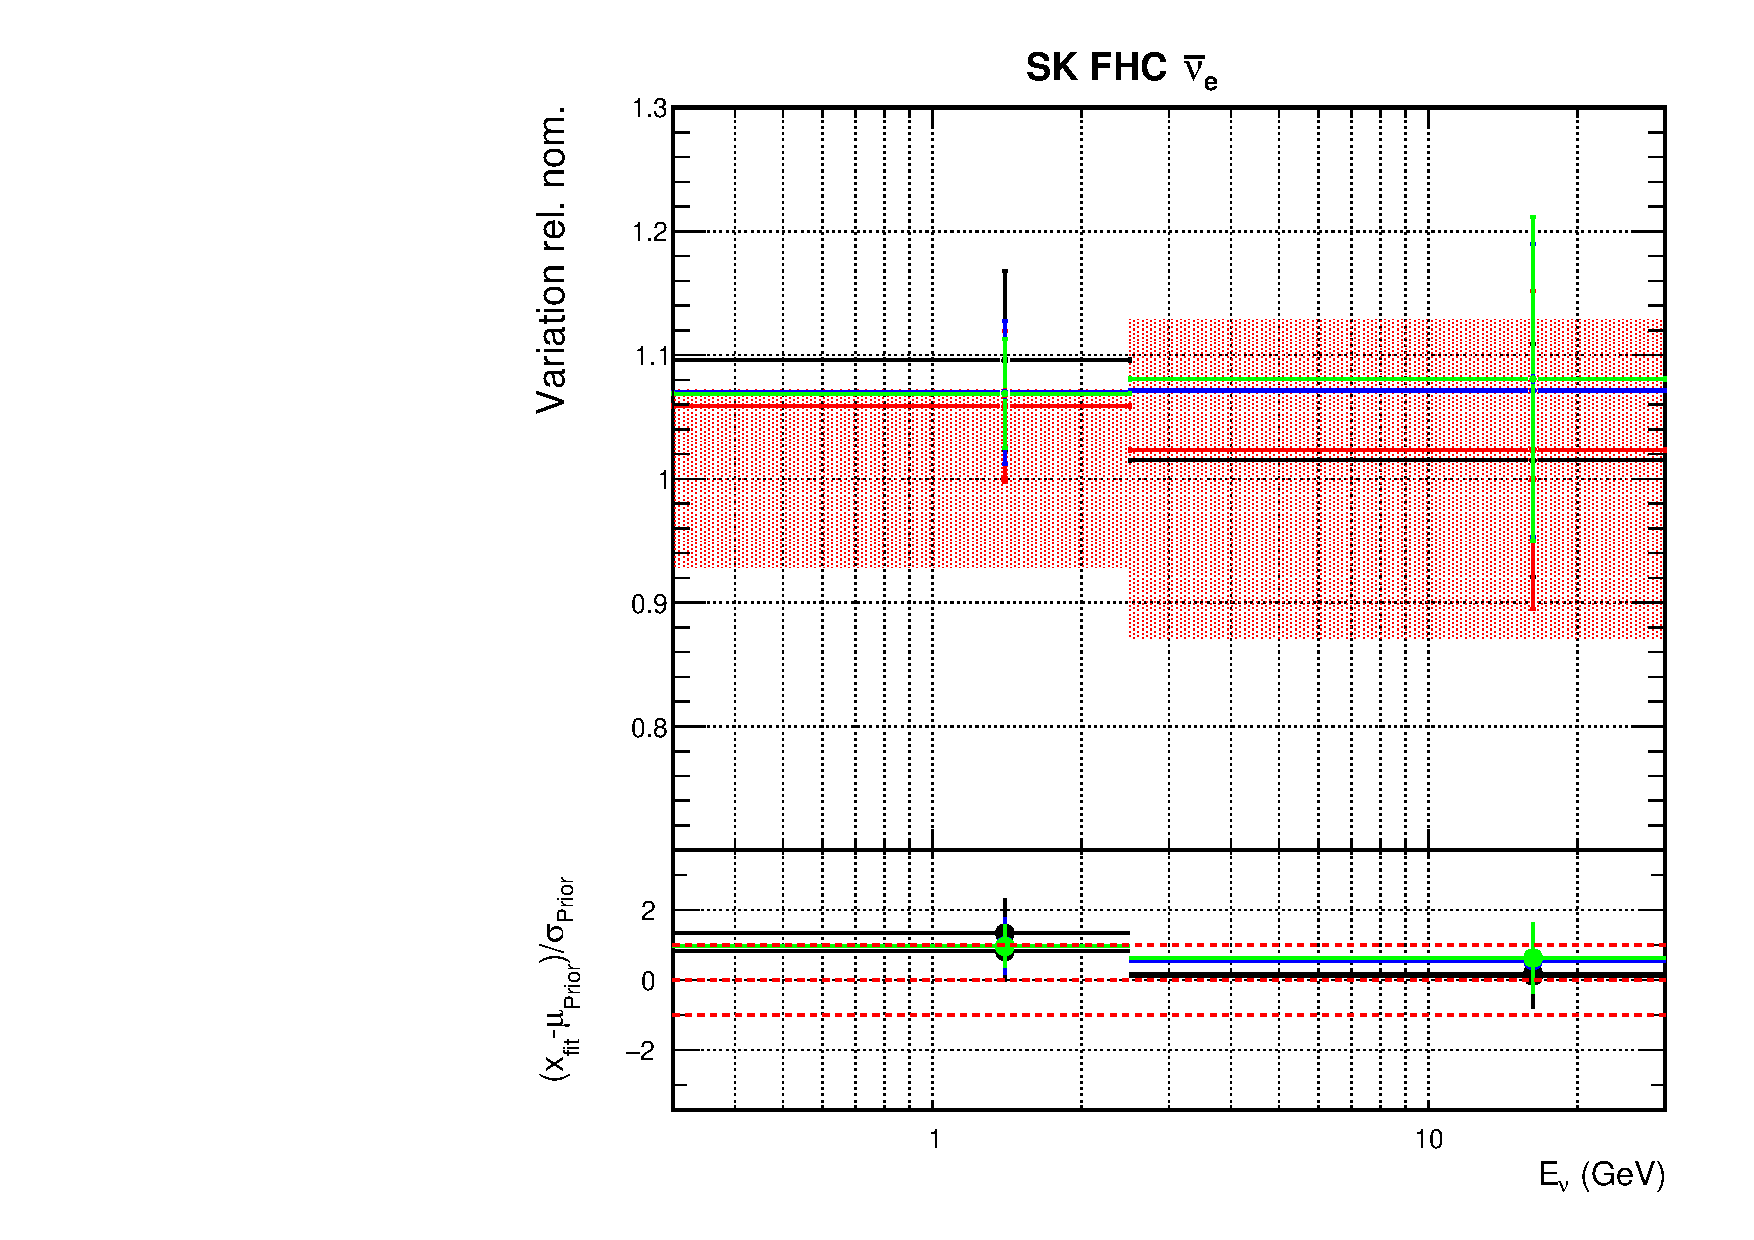
\includegraphics[width=0.75\linewidth]{figs/detcovbinflux_11}
  \caption{SK FHC $\bar{\nu_{e}}$}
\end{subfigure}
\begin{subfigure}{0.45\textwidth}
  \centering
  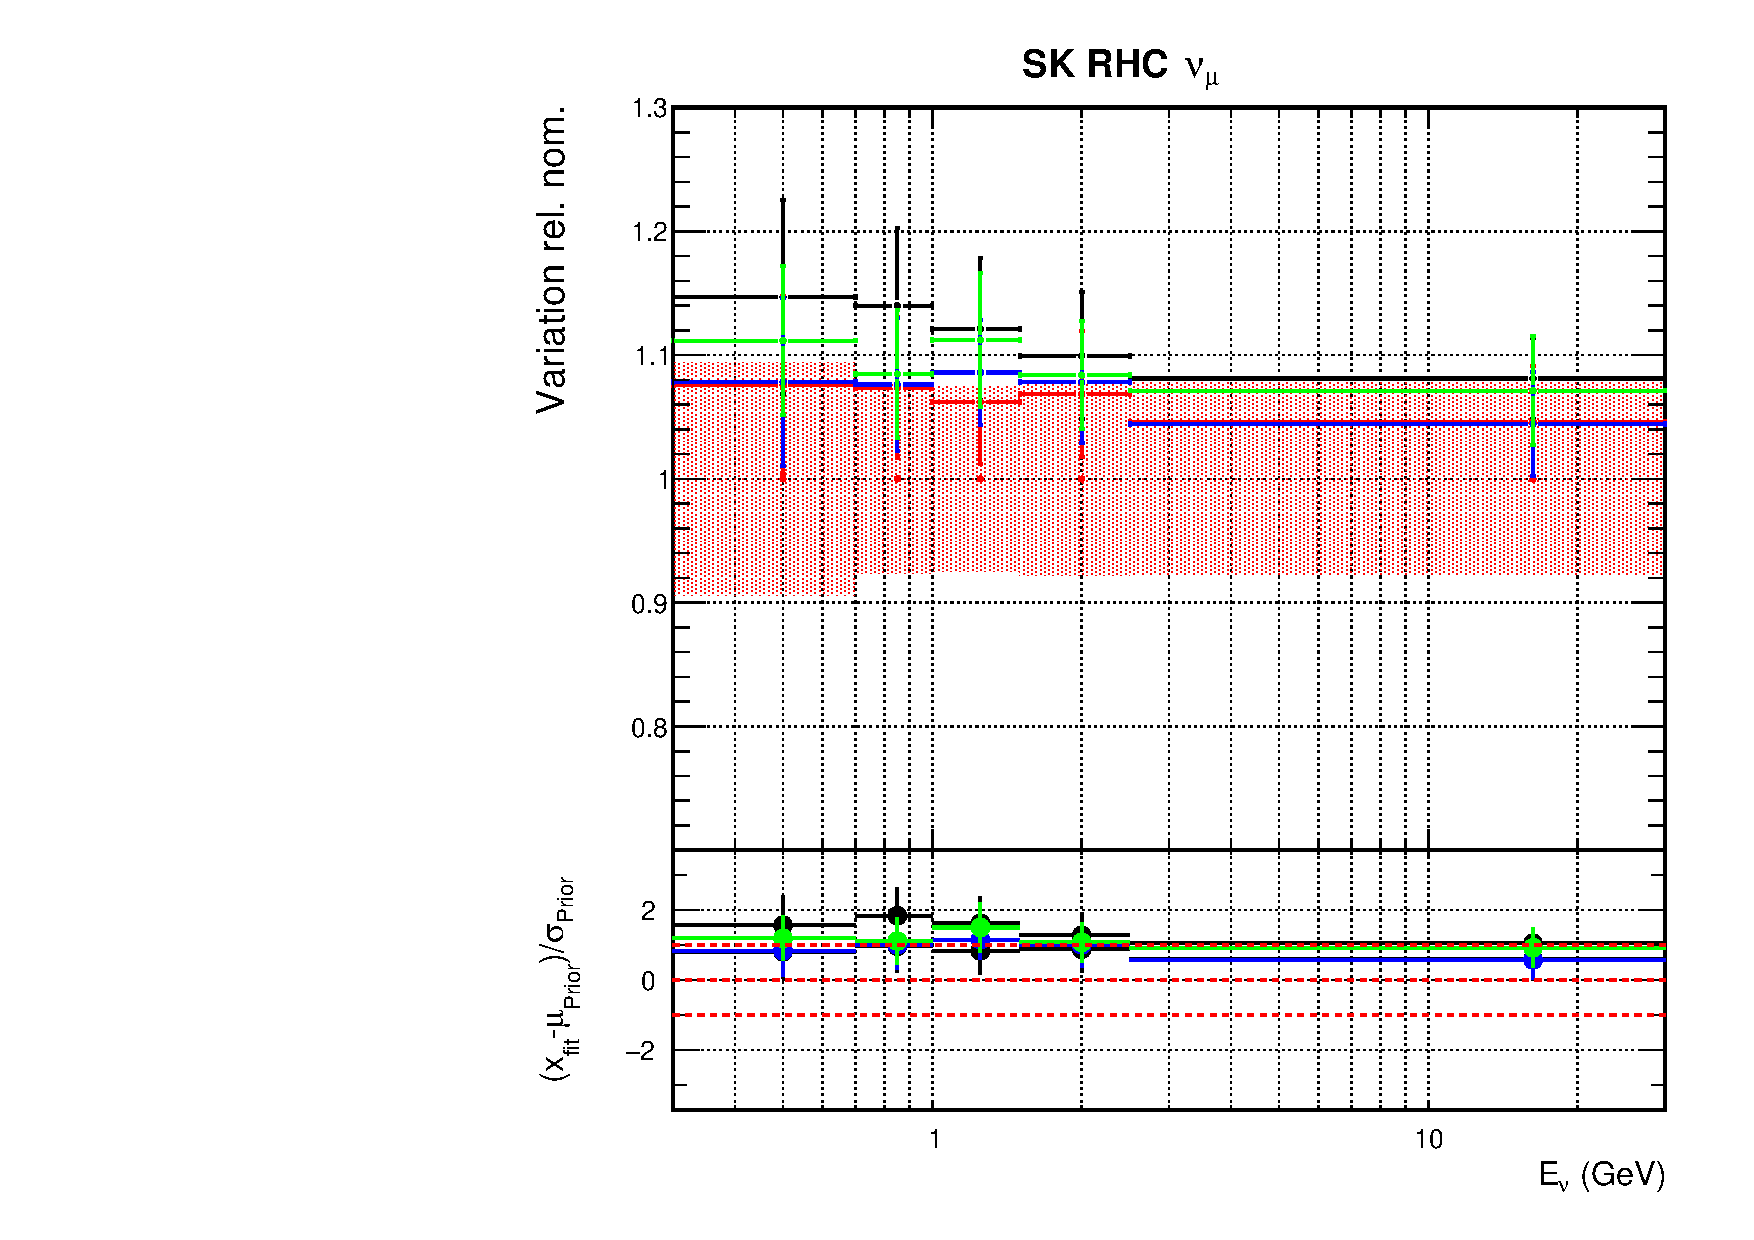
\includegraphics[width=0.75\linewidth]{figs/detcovbinflux_12}
  \caption{SK RHC $\nu_{\mu}$}
\end{subfigure}
\begin{subfigure}{0.45\textwidth}
  \centering
  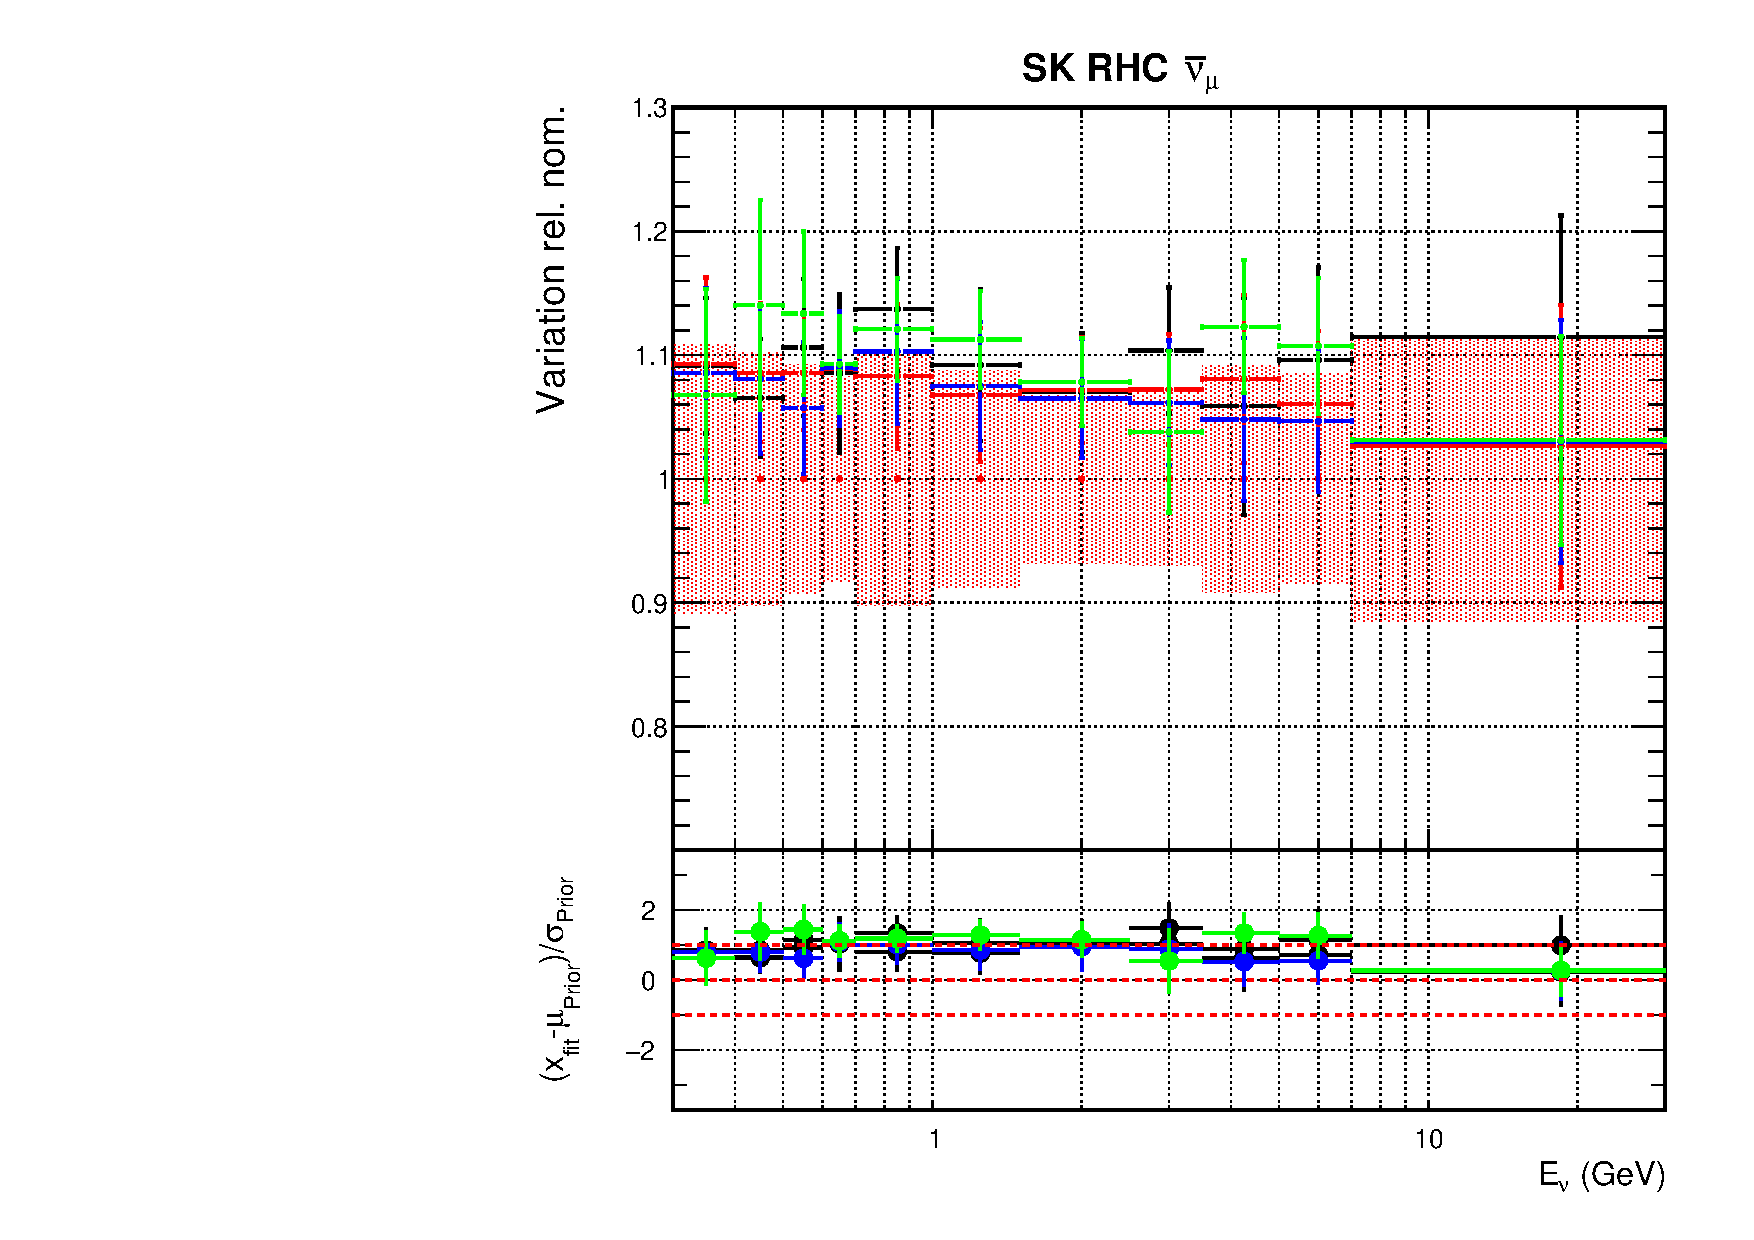
\includegraphics[width=0.75\linewidth]{figs/detcovbinflux_13}
  \caption{SK RHC $\bar{\nu_{\mu}}$}
\end{subfigure}
\begin{subfigure}{0.45\textwidth}
  \centering
  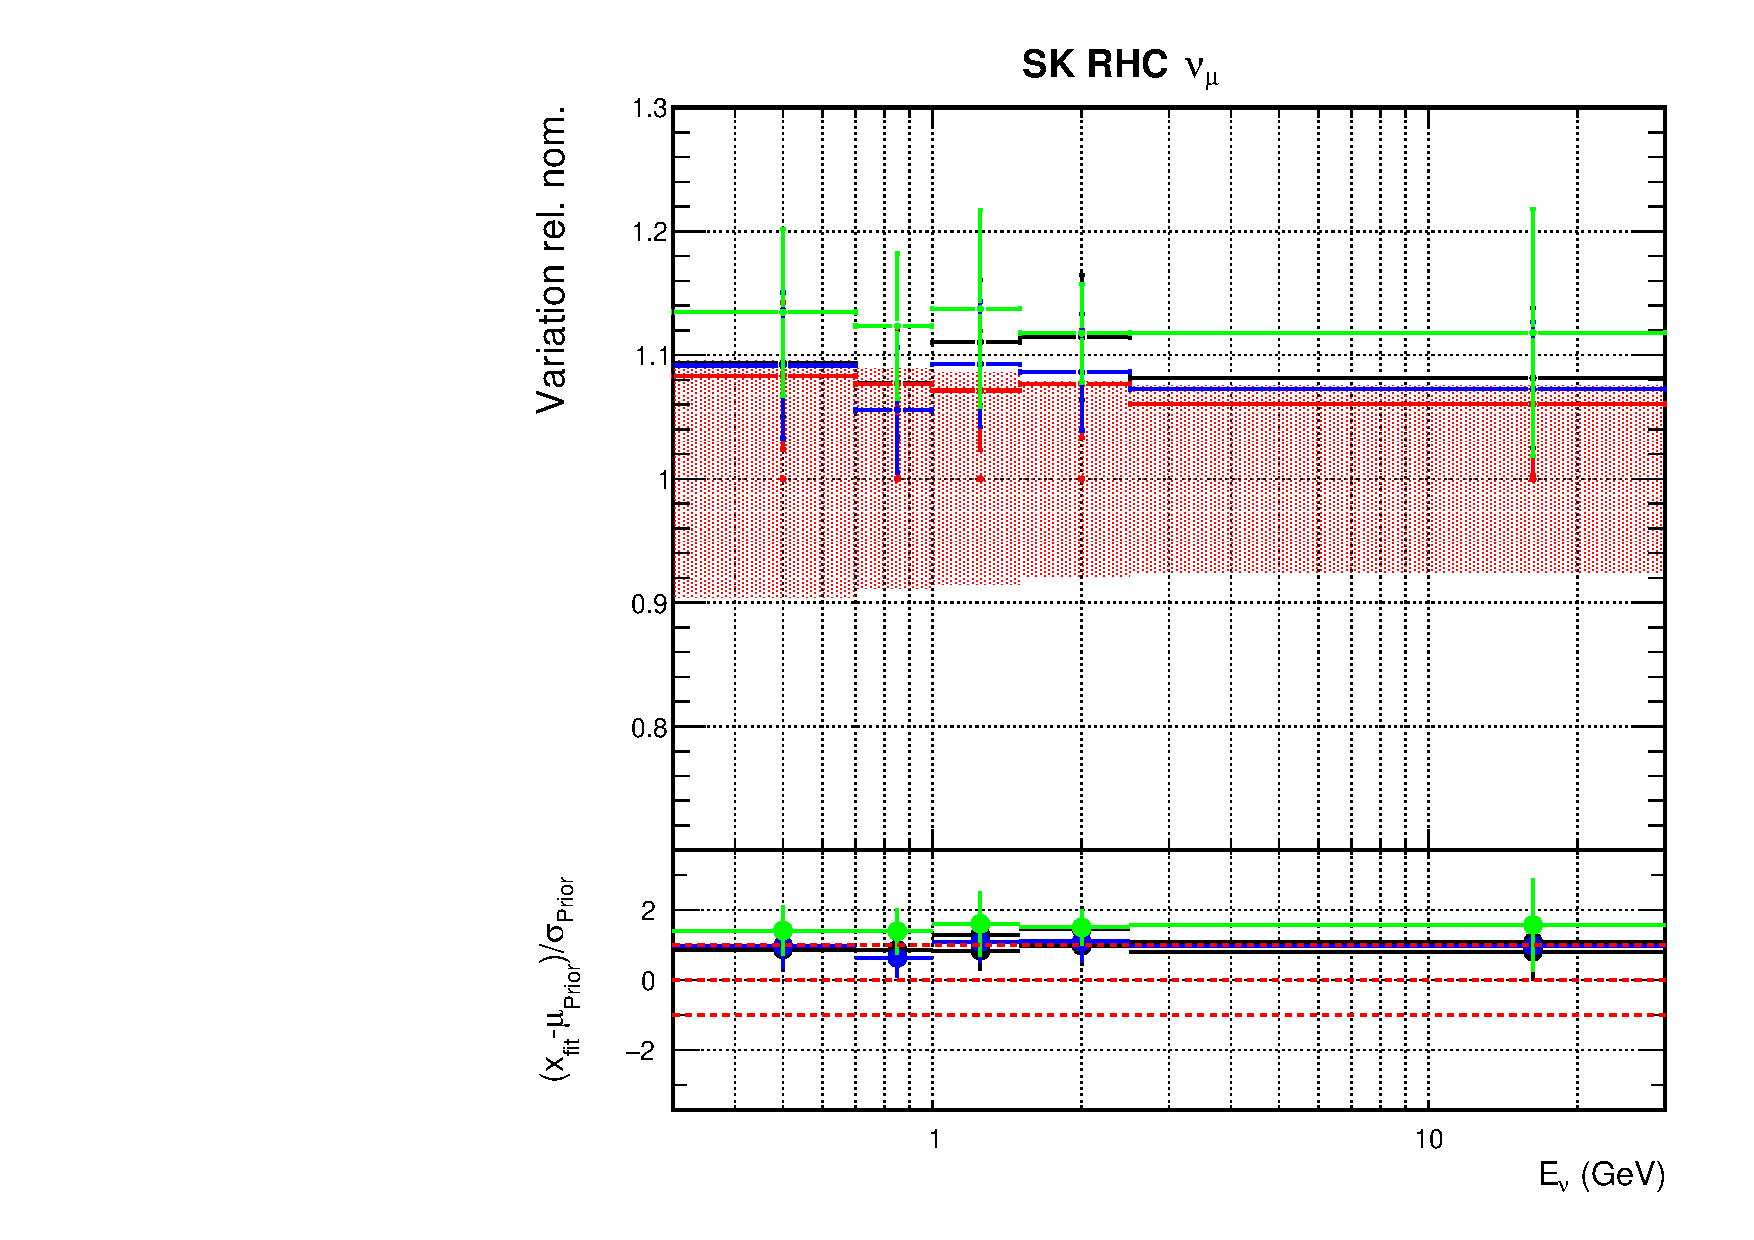
\includegraphics[width=0.75\linewidth]{figs/detcovbinflux_14}
  \caption{SK RHC $\nu_e$}
\end{subfigure}
\begin{subfigure}{0.45\textwidth}
  \centering
  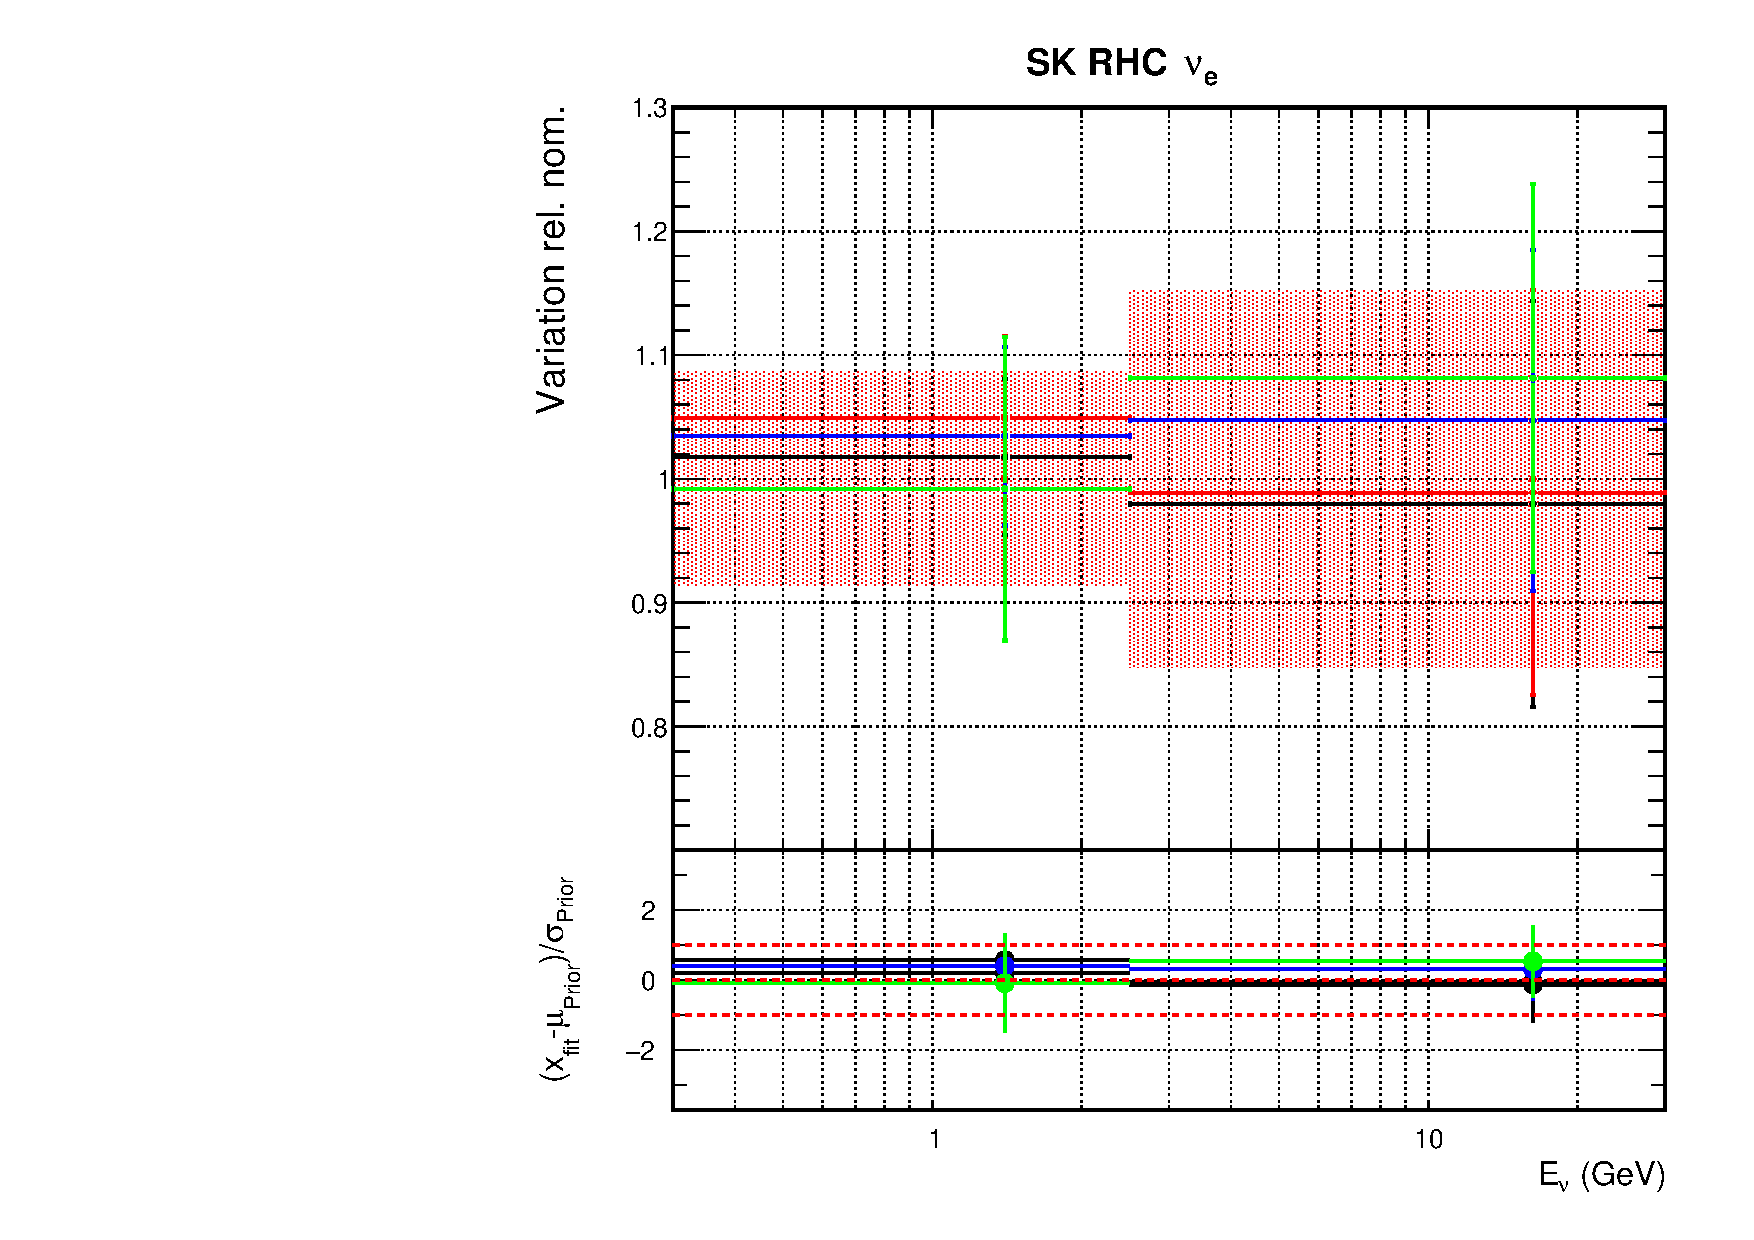
\includegraphics[width=0.75\linewidth]{figs/detcovbinflux_15}
  \caption{SK RHC $\bar{\nu_e}$}
\end{subfigure}
\caption{SK flux parameters for fake data fits using different detector binnings.}
\label{fig:detcovbinfluxSKapp}
\end{figure}

\begin{figure}[!htbp]
\centering
\begin{subfigure}{0.3\textwidth}
  \centering
  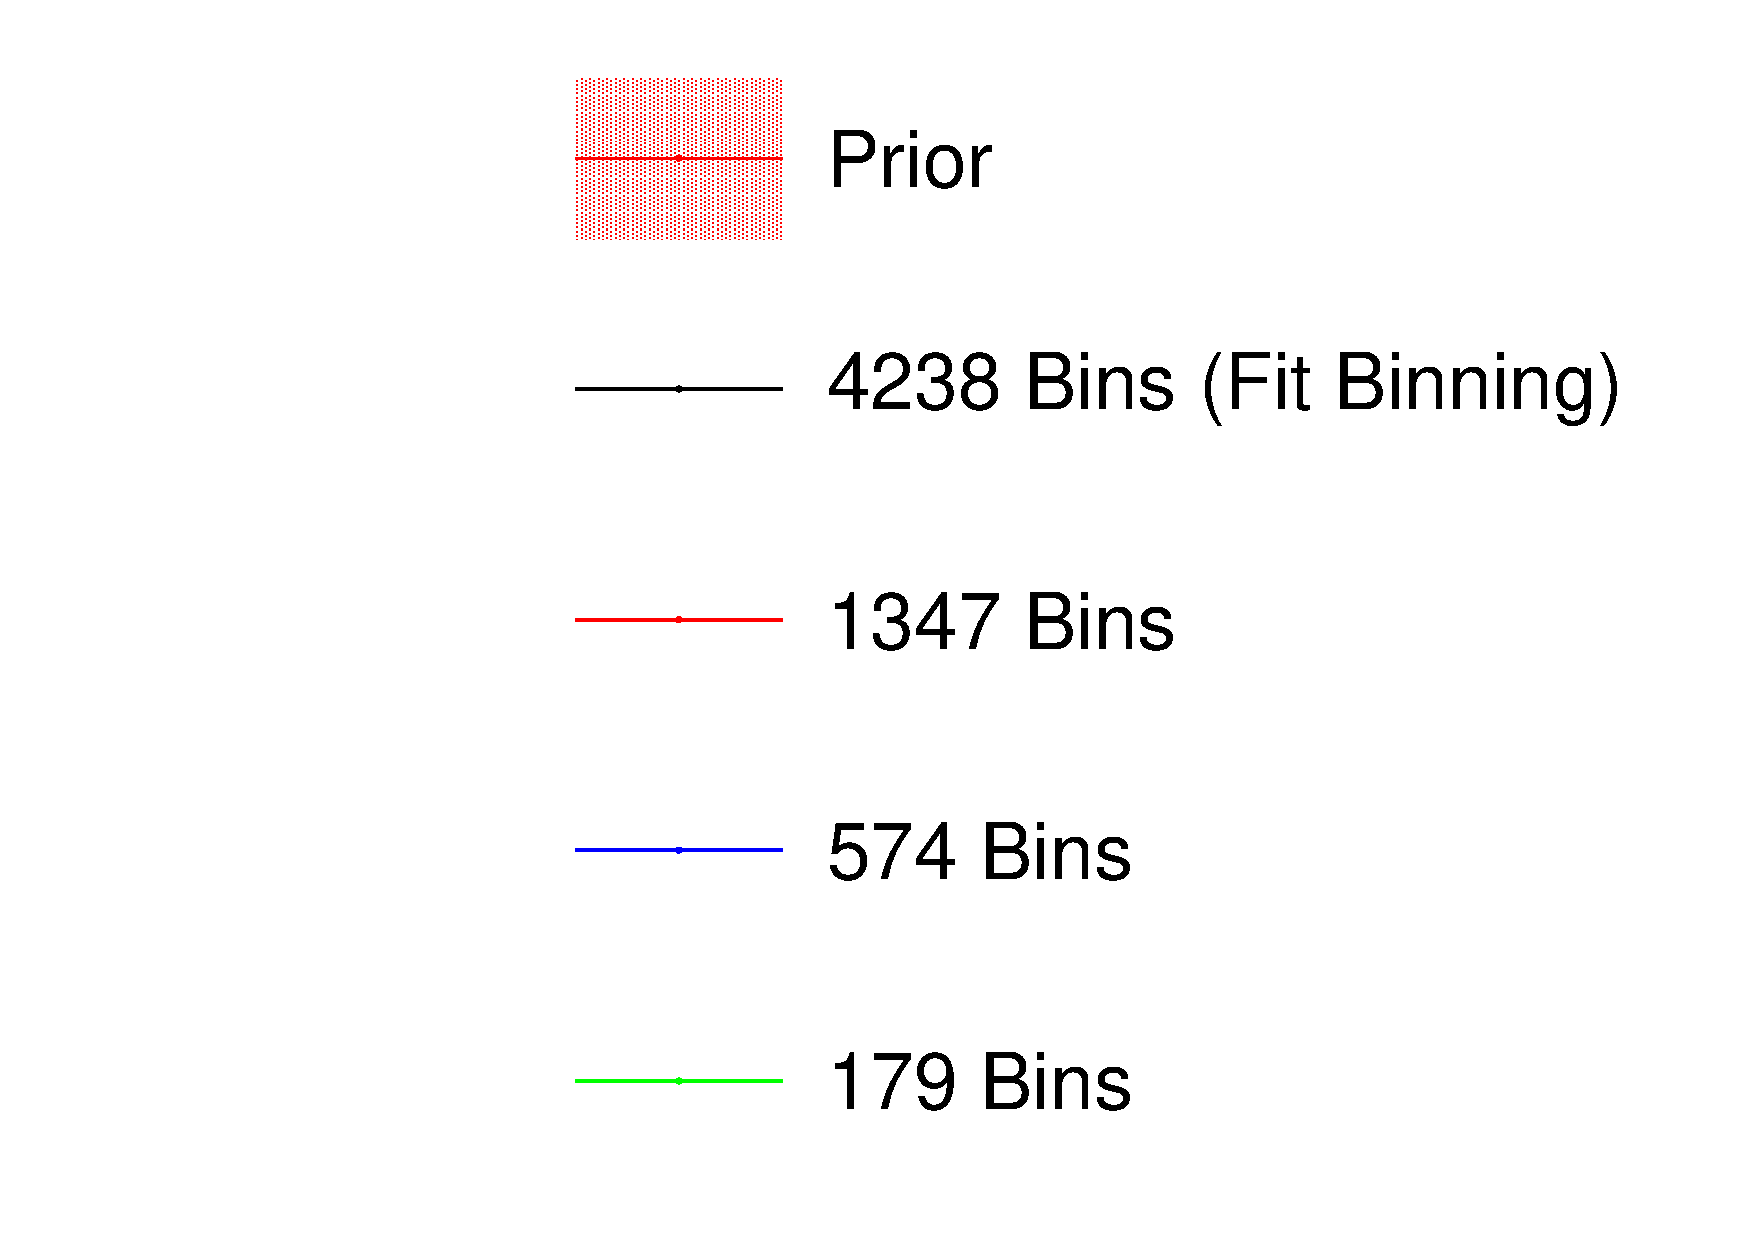
\includegraphics[width=0.8\linewidth, trim={5mm  65mm 0mm 0mm}, clip]{figs/detcovbin_leg}
\end{subfigure}
\begin{subfigure}{0.3\textwidth}
  \centering
  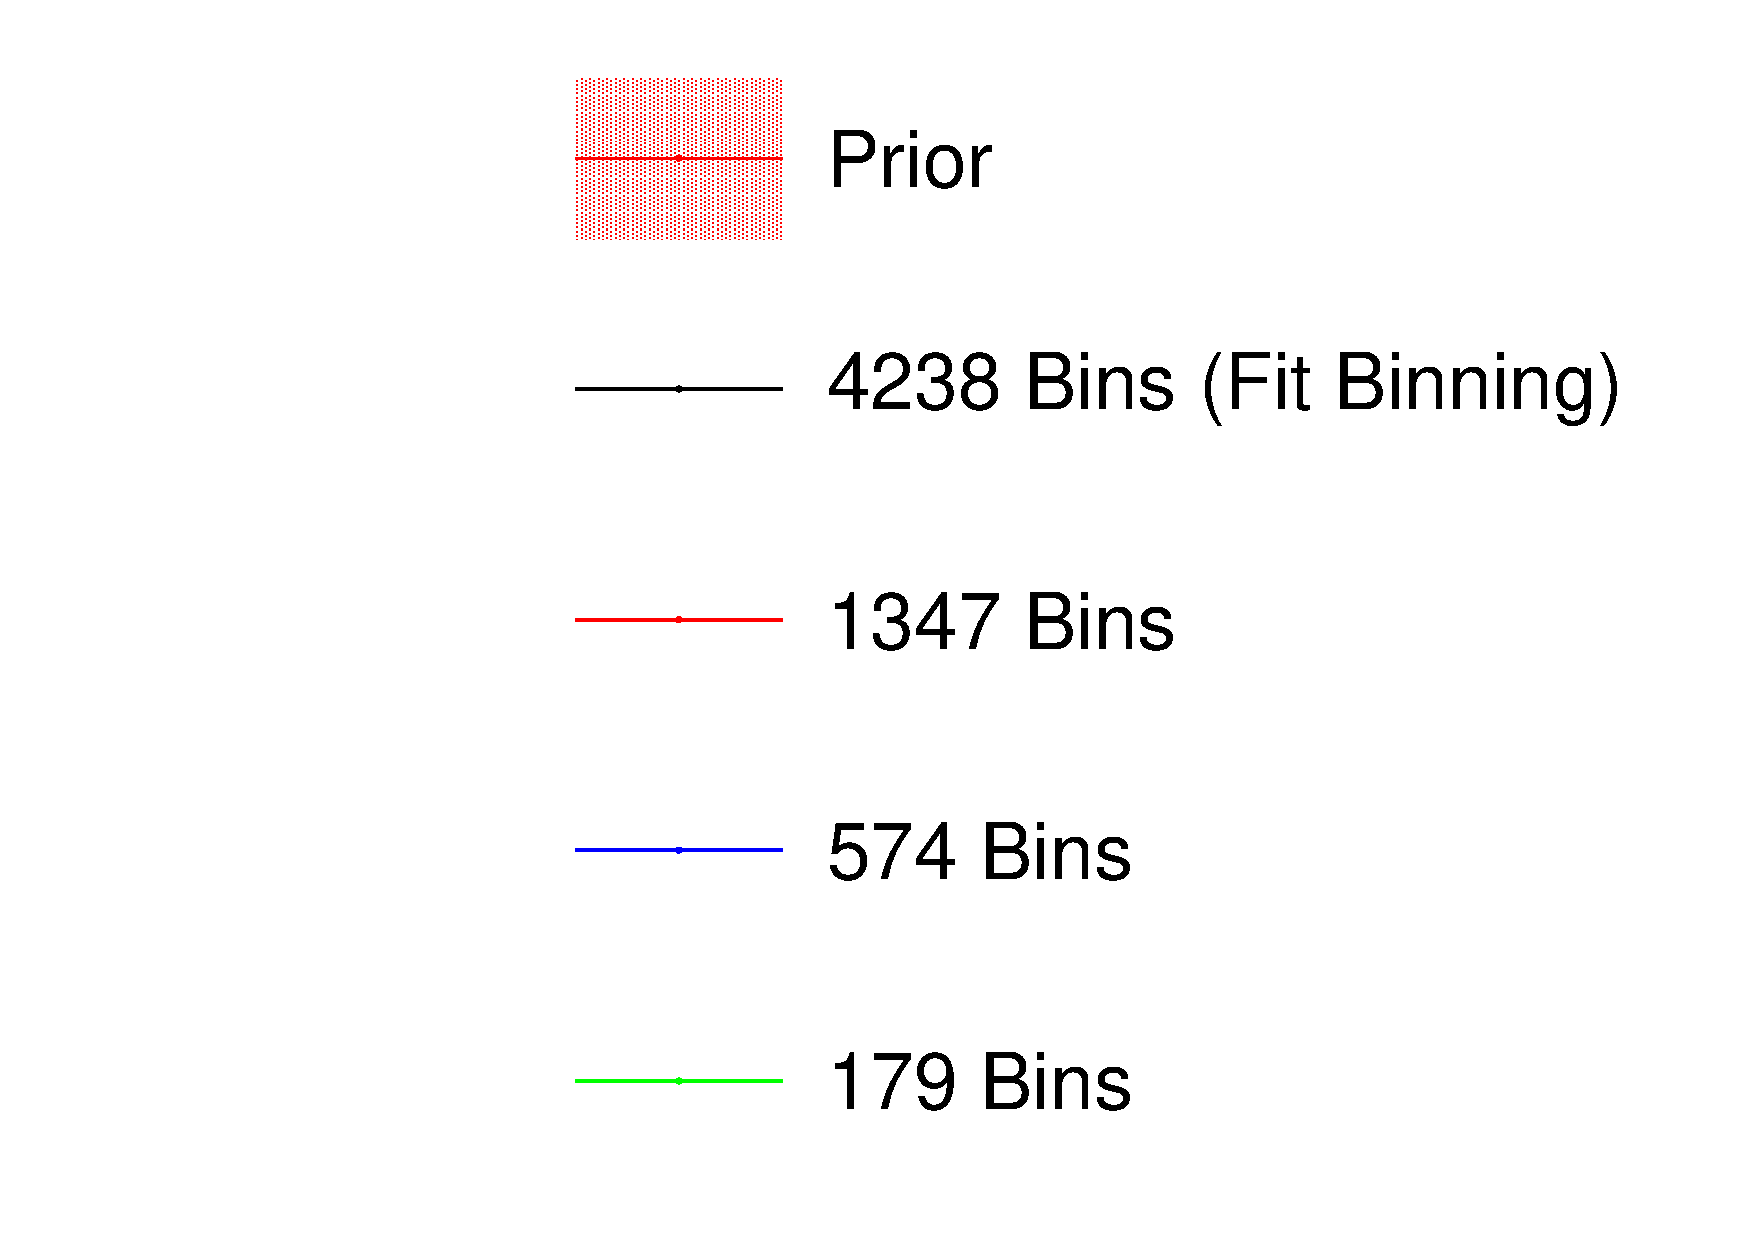
\includegraphics[width=0.8\linewidth, trim={5mm  0mm 0mm 105mm}, clip]{figs/detcovbin_leg}
\end{subfigure}
\begin{subfigure}{0.49\textwidth}
  \centering
  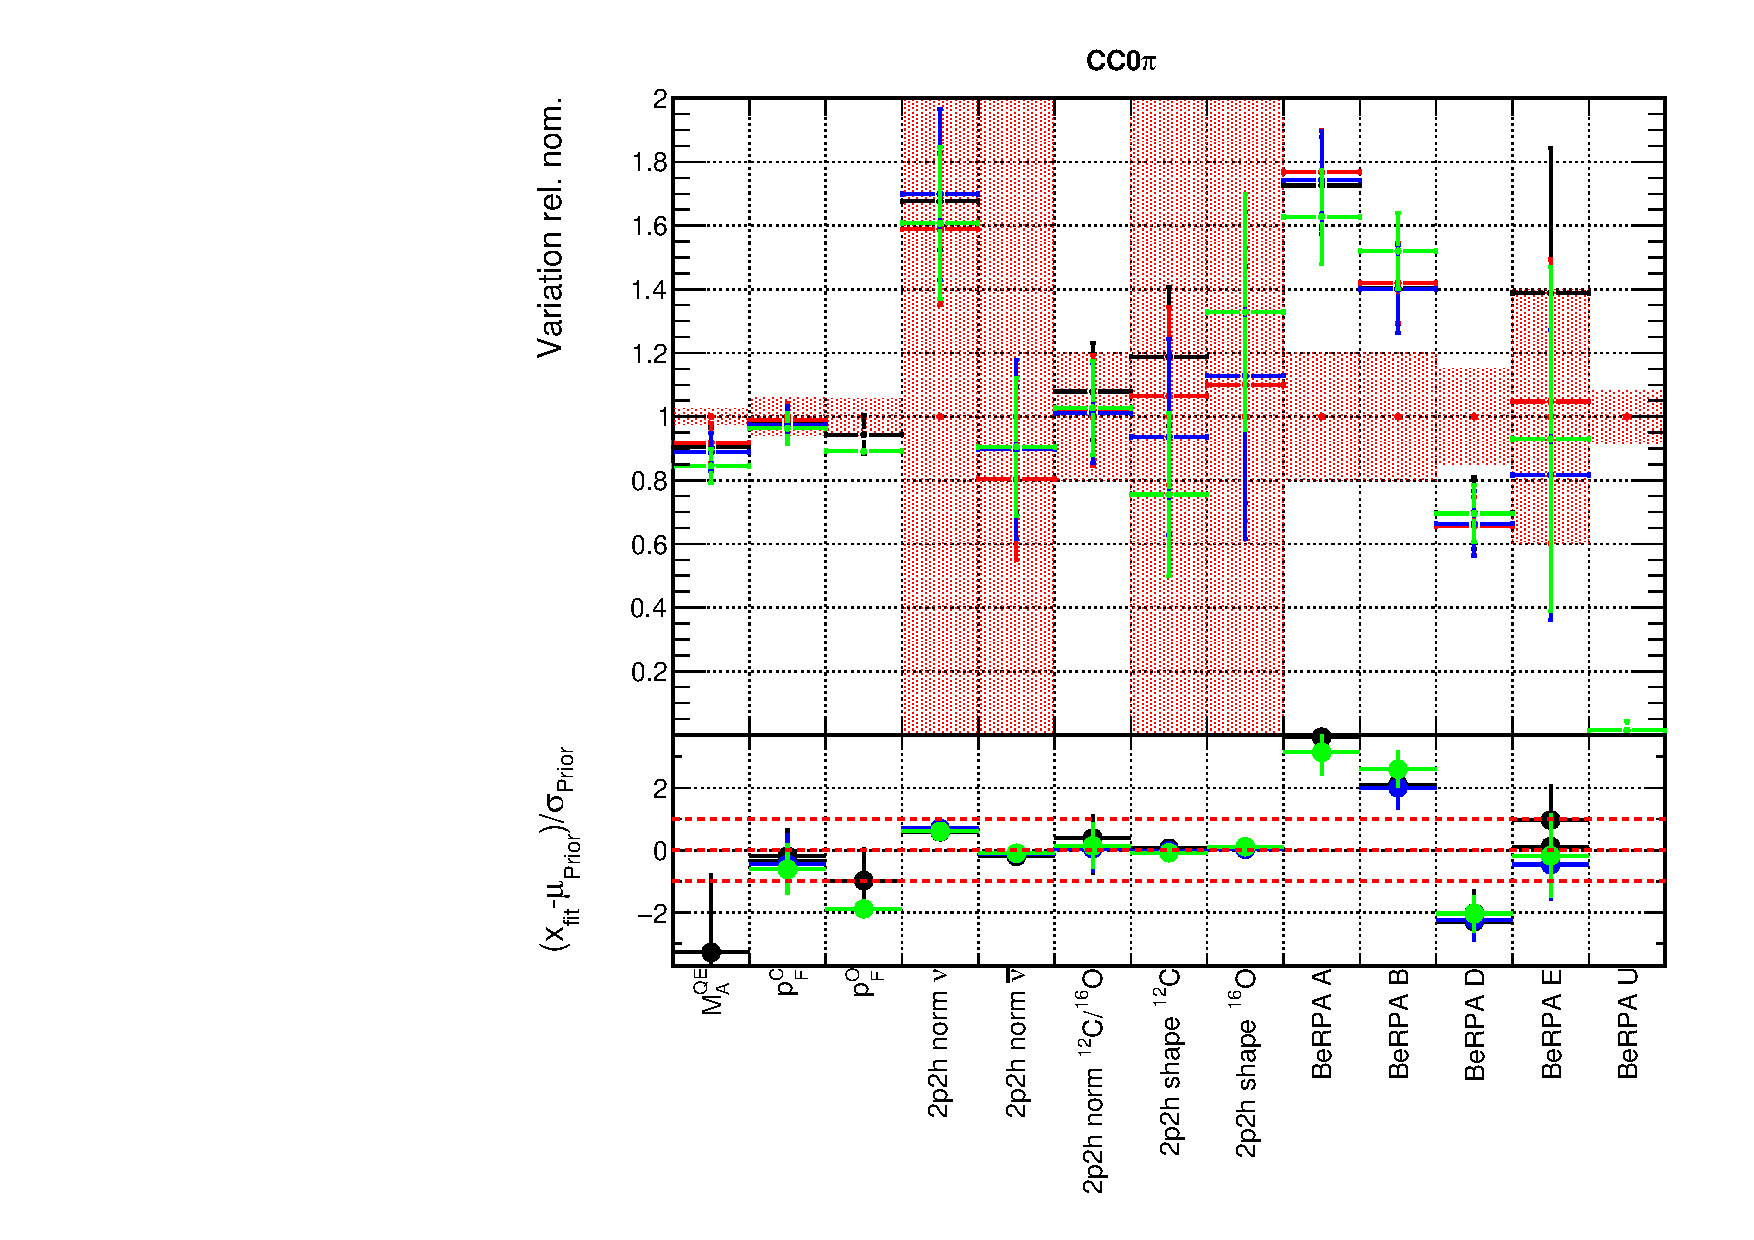
\includegraphics[width=0.95\linewidth]{figs/detcovbinxsec_1}
  \caption{CC0$\pi$}
\end{subfigure}
\begin{subfigure}{0.49\textwidth}
  \centering
  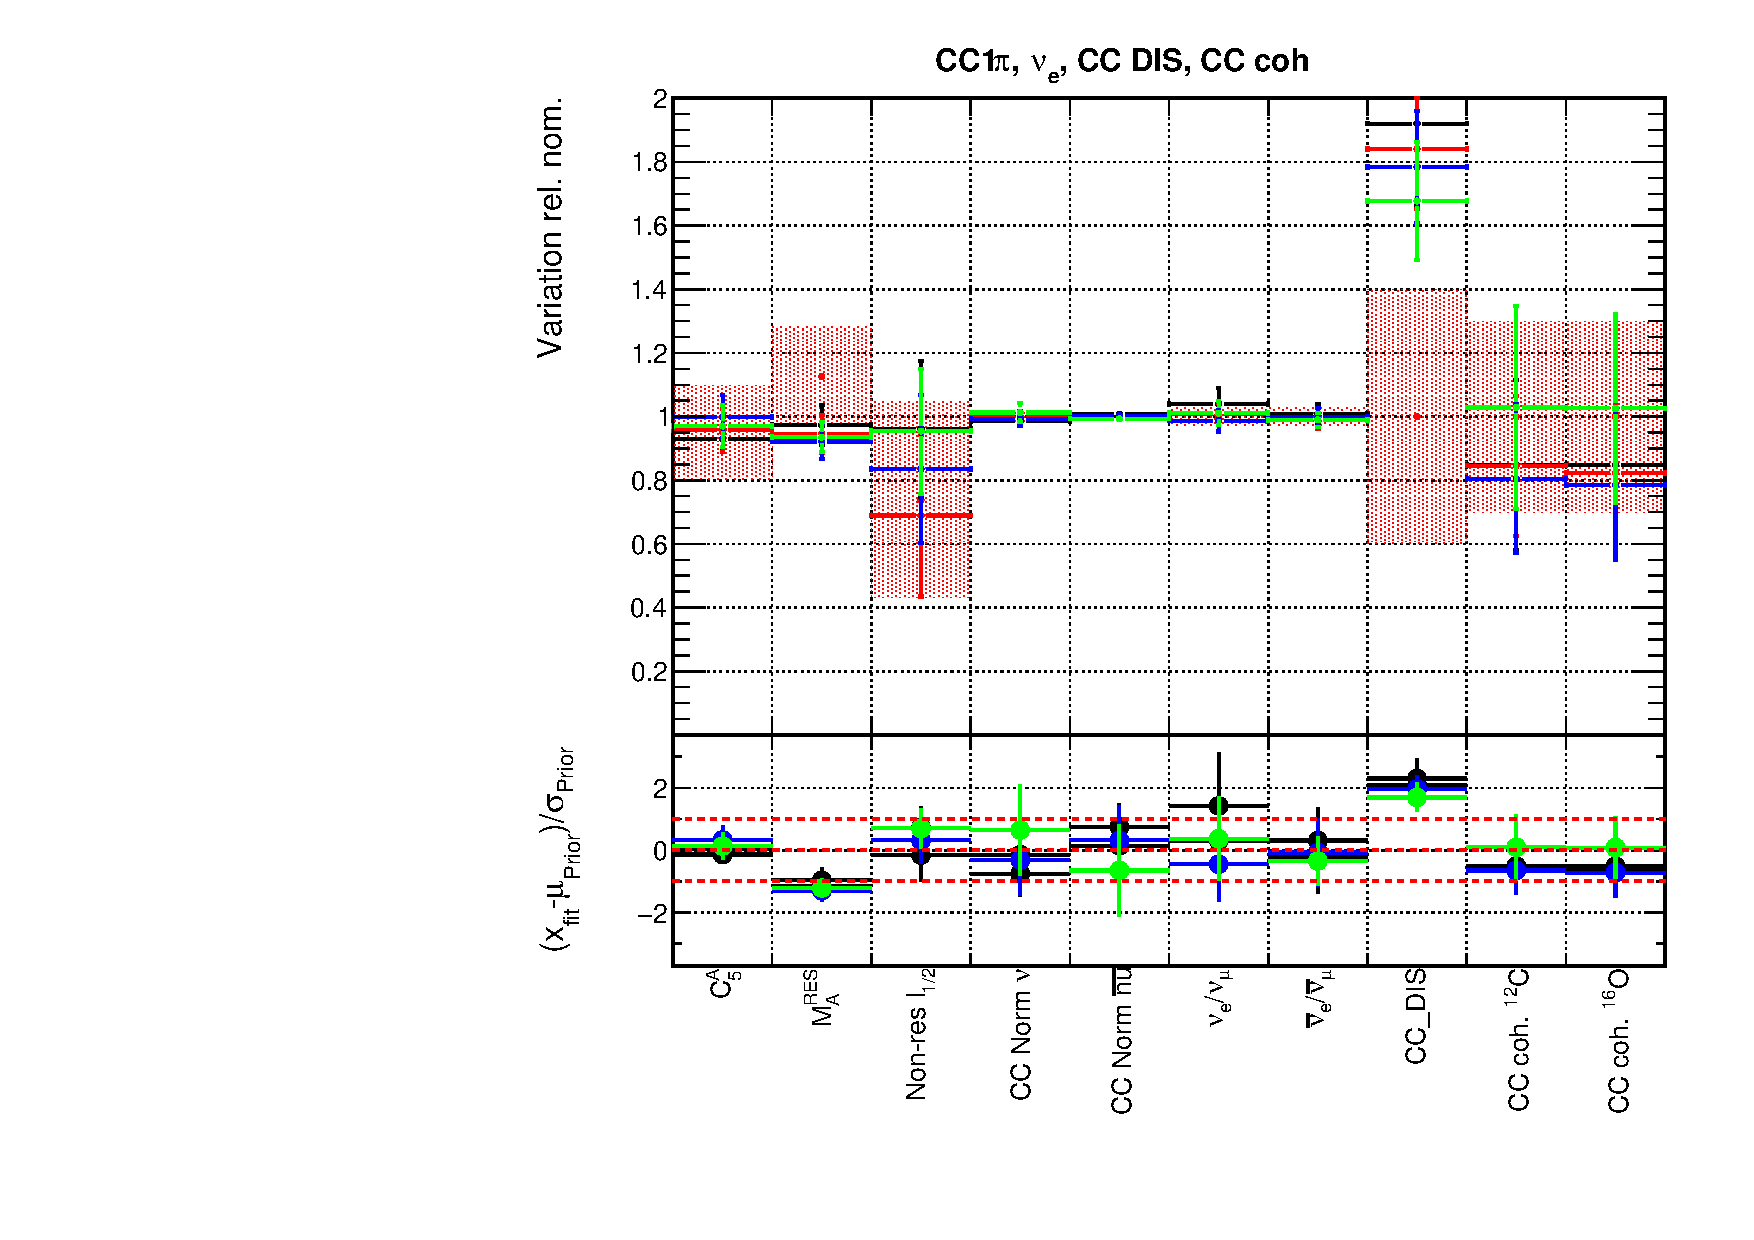
\includegraphics[width=0.95\linewidth]{figs/detcovbinxsec_2}
  \caption{CC1$\pi$, $\nu_e$, CC DIS, and CC coh.}
\end{subfigure}
\begin{subfigure}{0.49\textwidth}
  \centering
  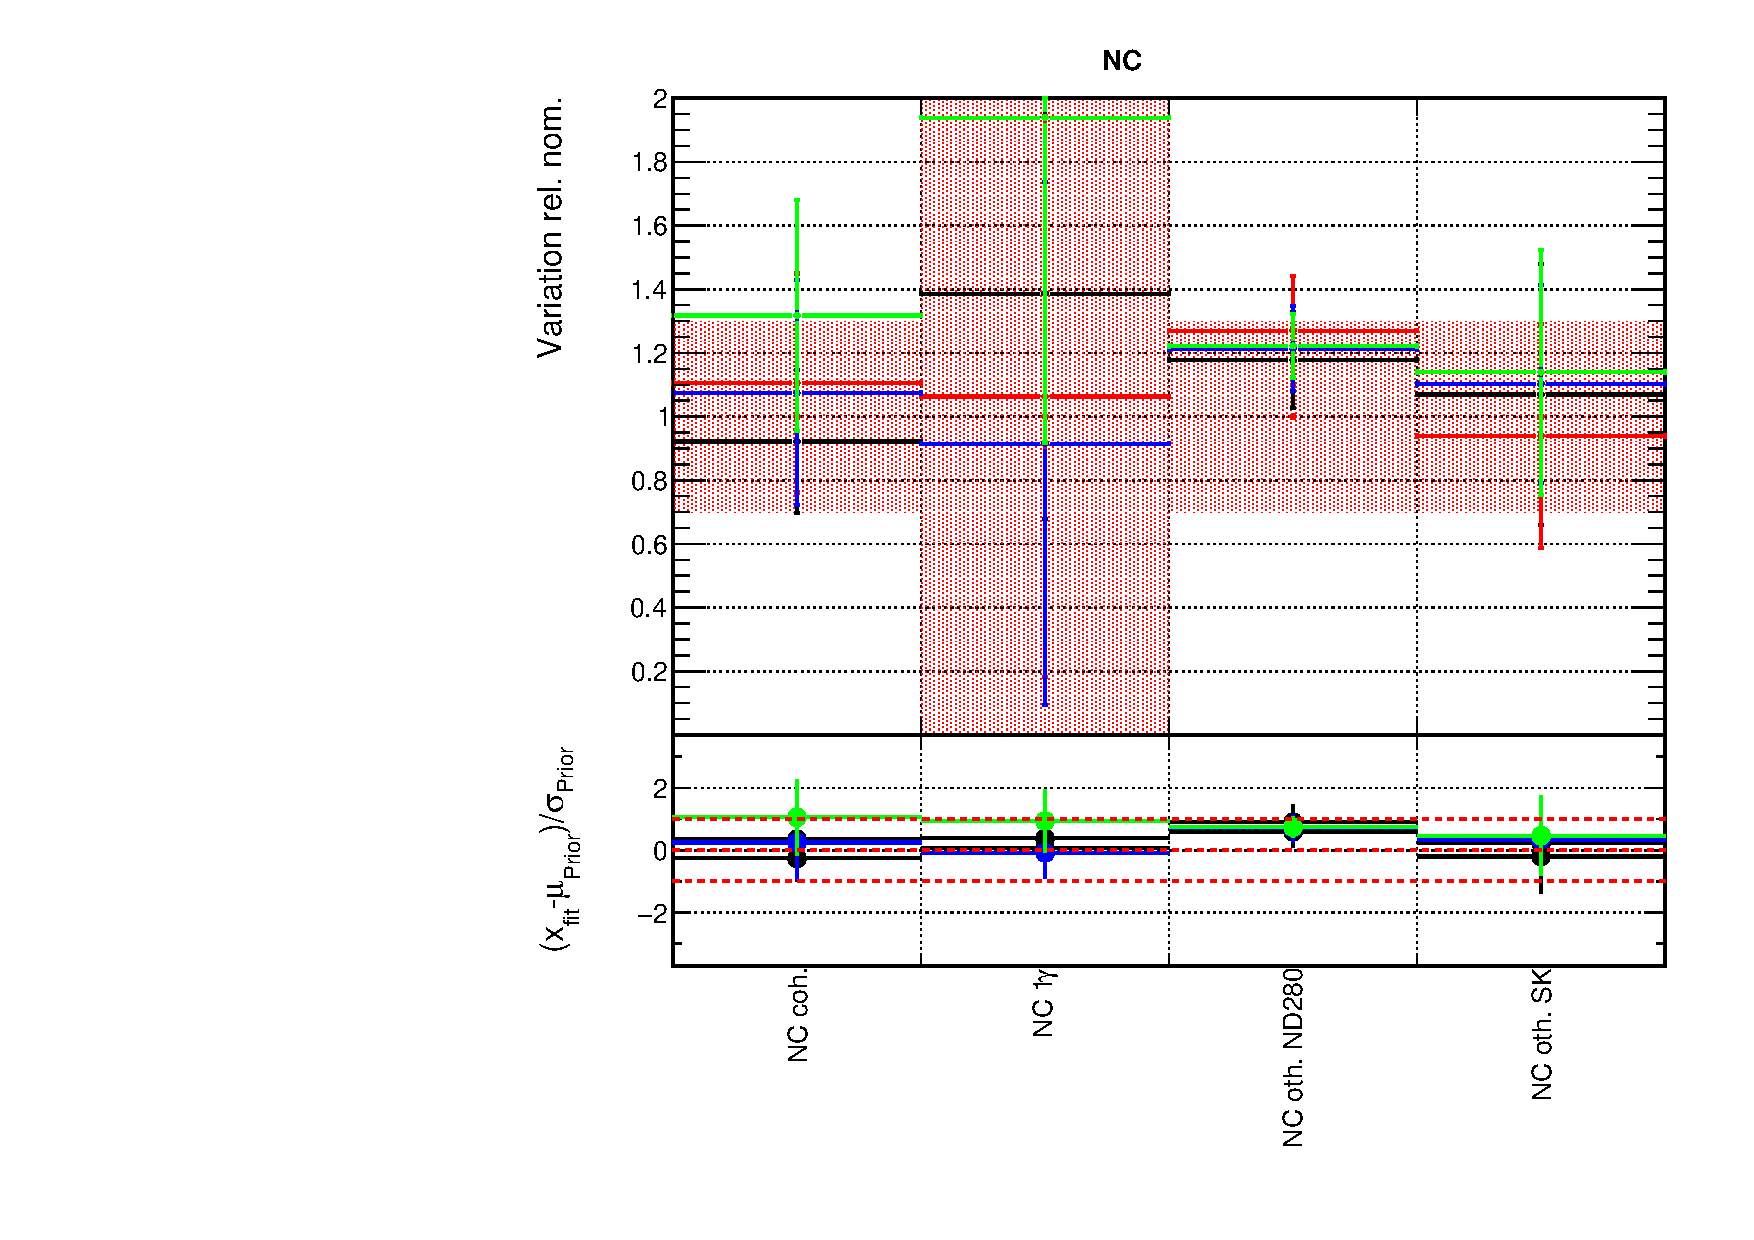
\includegraphics[width=0.95\linewidth]{figs/detcovbinxsec_3}
  \caption{NC.}
\end{subfigure}
\begin{subfigure}{0.49\textwidth}
  \centering
  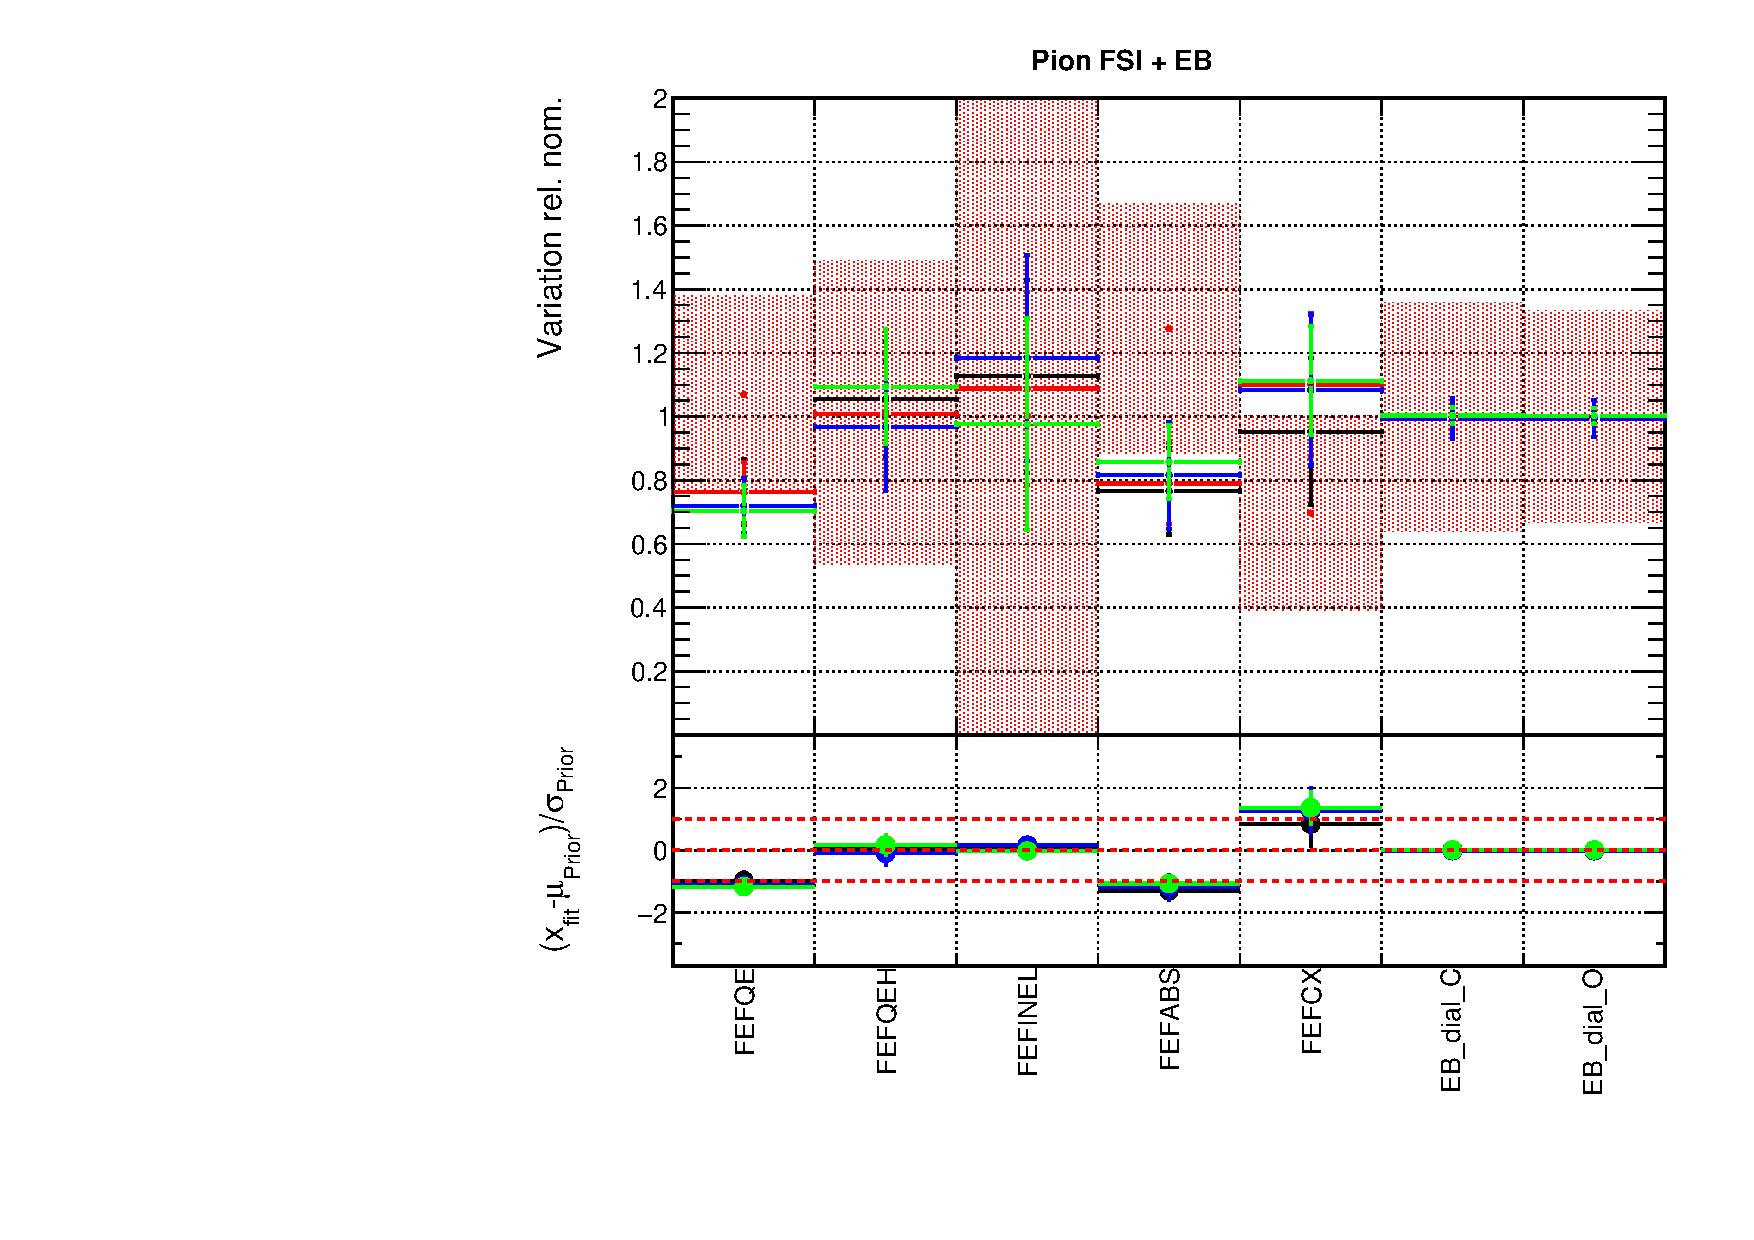
\includegraphics[width=0.95\linewidth]{figs/detcovbinxsec_4}
  \caption{$\pi$ FSI and $E_b$}
\end{subfigure}
\caption{Interaction parameters for fake data fits using different detector binnings.}
\label{fig:detcovbinxsecapp}
\end{figure}

\newpage